\documentclass[journal]{IEEEtran}
\usepackage[T1]{fontenc}
\usepackage{cite}
\usepackage{amsmath,amssymb}
\usepackage{graphicx}
\usepackage{booktabs}
\usepackage{adjustbox}
\usepackage{algorithm}
\usepackage{algpseudocode}
\usepackage{url}
\usepackage{textcomp}
\usepackage{tikz}
\usetikzlibrary{arrows.meta,fit,backgrounds,positioning}
\usepackage[hidelinks]{hyperref}
\hyphenation{Edge-IIoT-set Open-Flow Mini-net}

\begin{document}

\title{Federated Cascade Intrusion Detection for IIoT Networks: Poisoning-Resistant Aggregation, Connection-Level Evaluation and SDN Enforcement}

\author{Aaryan~Prakash,
        Aaron~B~Ajay,
        Amal~Roy,
        and~Amogh~Krishna~J~S%
\thanks{The authors are with the Department of Computer Science \& Engineering, BMS College of Engineering, Bengaluru, Karnataka, India.}}

\markboth{Preprint, November 2026}{Prakash \MakeLowercase{\textit{et al.}}: Federated Cascade Intrusion Detection for IIoT Networks}

\maketitle

\begin{abstract}
IoT and IIoT sites rarely want to send raw traffic to a central detector, and a detector trained only on labelled attacks cannot recognise an attack type it has never seen. Federated learning keeps traffic local but lets any site send a poisoned update. We present FL-IDS: a LightGBM classifier names known attacks, a per-site autoencoder flags traffic unlike benign traffic, federated training uses a trust filter and trimmed-mean aggregation, and verdicts become OpenFlow~1.3 rules in an emulated network. We test the whole system on all 1,985,768 unique rows of Edge-IIoTset with every connection kept on one side of every split, after correcting three defects in the released data: a placeholder-spelling label leak (reported independently by Galal), column-shifted MITM rows, and a \texttt{tshark} version difference that zeroes a feature in live extraction. In six real multi-process runs the cascade detects 99.39 to 99.81\% of known attacks (macro-recall). Packet false alarms are 2.5 to 16.3\%, but 0.34 to 1.04\% per benign connection. On attack types withheld from training the cascade detects 0.895 to 0.944 on average, against 0.723 to 0.757 for the classifier alone. With 30\% sign-flipping sites the filter keeps the autoencoder working where plain averaging destroys it, but it admits attackers in 50 to 62\% of their rounds and fails at 50\%. Replaying all 14 attack captures ends in a verified drop rule each time, with 12 named correctly. Among 15 classifiers, tree models are interchangeable on the final 130 features (macro F1 0.979 to 0.985), while boosting leads on the 91 base features.

\end{abstract}

\begin{IEEEkeywords}
Federated learning, intrusion detection, IIoT, Byzantine robustness, autoencoder, gradient boosting, software-defined networking, dataset leakage, Edge-IIoTset.
\end{IEEEkeywords}

\section{Introduction}
\label{sec:intro}
Machine-learning intrusion detection for IoT and industrial IoT (IIoT) networks usually assumes that traffic from every site can be pooled in one place. The operators of a plant floor, a hospital wing or a building network often cannot send packet data off-site, for privacy, contractual or bandwidth reasons. Federated learning (FL)~\cite{mcmahan2017} avoids the transfer: each site trains on its own traffic and shares only model parameters. FL-based intrusion detection is by now an established area with its own systematic review~\cite{hernandez2025}, so a federated detector on its own is not a contribution. A system that could be deployed still has to deal with five problems at once.

\textbf{1. Known and unknown attacks.} A supervised classifier names only the classes it was trained on. A new attack type is assigned to its nearest known class or to benign. An unsupervised detector flags departures from benign traffic, but cannot say what kind of attack it found.

\textbf{2. Poisoned updates.} Any site in a federation can send any update it likes. Byzantine-robust aggregation~\cite{blanchard2017,yin2018,cao2021fltrust} limits the damage, but its performance drops when site data are non-IID~\cite{li2024experimental}, which is the normal case for IoT, because honest heterogeneous sites and attackers both look like outliers.

\textbf{3. Enforcement.} A detection that nobody acts on does not stop the attack. Software-defined networking (SDN)~\cite{mckeown2008} provides a programmable point of enforcement.

\textbf{4. Data integrity.} Results on a public dataset are only as sound as its released files. Preprocessing artifacts that encode the label make published numbers unreliable~\cite{galal2026,arp2022,engelen2021}.

\textbf{5. Evaluation scale and leakage.} Packets of one connection share much of their information. A test set that contains packets from connections also seen in training rewards memorising connections, and evaluations on small subsamples hide how a federated system behaves with realistic data volumes.

This paper describes FL-IDS, a system built to address all five in one pipeline, and reports what each part contributes when measured on its own. A LightGBM~\cite{ke2017} classifier labels known attack types first. Traffic it labels benign, or labels as an attack with low confidence, passes to an autoencoder at the site, whose reconstruction error flags anything unlike benign traffic. This ordering follows a centralised two-stage design by Zhang et al.~\cite{zhang2023twostage}. Here the autoencoder is trained federatedly with Flower~\cite{beutel2020}, and a server-side trust filter screens the sites' updates before a trimmed-mean aggregation. The combined verdict drives OpenFlow~1.3 flow rules in an emulated network. The choice of boosting for the first stage rests on a model-selection study that ran in three earlier stages of the project and was repeated on Edge-IIoTset for this paper (Section~\ref{sec:models}).

\subsection*{Contributions}
\begin{itemize}
  \item \textbf{An integrated federated IDS} that combines a boosting-first detection cascade, a federated autoencoder, an update-level trust filter and SDN enforcement. Section~\ref{sec:related} compares it with the closest published systems; each covers some of these parts, and none we found covers all of them.
  \item \textbf{An evaluation of the whole system on all 1,985,768 unique rows of Edge-IIoTset}~\cite{ferrag2022}, with every connection kept whole on one side of every split. It includes six real multi-process training runs (10 and 20 sites, three seeds), an ablation and a poisoning sweep over three seeds, a leave-one-class-out test for all 14 attack types over three seeds, and replays of all 14 attack captures through the SDN path.
  \item \textbf{A measurement of how false alarms should be counted.} Counted per packet, false alarms are dominated by a few very long benign connections. Counted per connection, the rate is between 5.7 and 38 times lower.
  \item \textbf{Three corrections to Edge-IIoTset.} A placeholder-spelling leak that lets one feature separate benign from attack traffic perfectly (found independently of Galal~\cite{galal2026}, who reports the same mechanism), a set of MITM rows whose values sit under the wrong column names, and a \texttt{tshark} version difference that silently zeroes a feature in live extraction. To our knowledge the last two have not been reported.
  \item \textbf{A feature study} showing that the dataset's 91 standard features cap any classifier that sees only them at 0.969 macro recall, and that adding a service port, numeric payload-content features and connection-level aggregates lifts LightGBM to 0.983--0.985 macro F1 on connections it never saw in training.
  \item \textbf{A model-selection study} in three stages: two earlier stages on other datasets (MQTTset, DataSense) and a broad comparison of tree ensembles, linear, instance-based and neural classifiers on Edge-IIoTset, which gives the evidence for choosing boosting as the first stage.
  \item \textbf{Tests of the trust filter} against a white-box attacker that knows its rules, of pruning the autoencoder during and after training, and of a time-ordered split.
\end{itemize}

Section~\ref{sec:related} reviews related work. Section~\ref{sec:data} covers the dataset, its defects and the feature set. Section~\ref{sec:system} presents the system and Section~\ref{sec:setup} the experimental setup. Section~\ref{sec:results} reports the system results and Section~\ref{sec:models} the model-selection study. Section~\ref{sec:discussion} discusses the results and lists the limitations, and Section~\ref{sec:conclusion} concludes.

\section{Related Work}
\label{sec:related}
\subsection{Federated intrusion and anomaly detection}
Hern{\'a}ndez-Ramos et al.~\cite{hernandez2025} review FL-enabled IDS work from 2018 to 2022 and classify it by model, dataset, aggregation function and library. Mothukuri et al.~\cite{mothukuri2022} run federated training rounds on GRU models for IoT anomaly detection. DeepFed~\cite{li2021deepfed} trains a combined CNN and GRU classifier across industrial cyber-physical sites. Neither includes a supervised stage plus an unsupervised stage for traffic outside the trained label set.

Autoencoders appear in several federated designs. Rey et al.~\cite{rey2022} train both a supervised MLP and an unsupervised autoencoder across IoT devices for malware detection. They also show that plain averaging is badly exposed to malicious participants and test alternative aggregation functions as countermeasures. FedMSE~\cite{nguyen2025fedmse} pairs a shrink autoencoder with a centroid one-class classifier and weights each local model by its error during aggregation. Kitsune~\cite{mirsky2018} showed earlier that an ensemble of autoencoders can detect network intrusions online without supervision. The closest system to ours on the FL side is TA-FHIDF~\cite{sazid2026}. It combines an autoencoder, a 1D-CNN and a BiLSTM at the edge, scores client reliability by cosine similarity before global aggregation, and evaluates on UNSW-NB15, CICIDS2017 and Edge-IIoTset. As described in its abstract, it has no supervised-first cascade and does not mention network enforcement.

\subsection{Byzantine-robust aggregation}
Krum~\cite{blanchard2017} chooses the update closest to its neighbours. Coordinate-wise median and trimmed mean~\cite{yin2018} bound the influence of any single client on each coordinate, but only up to their breakdown point: a trimmed mean that cuts $k$ updates from each side cannot absorb more than $k$ colluding attackers. Fang et al.~\cite{fang2020} showed that attackers who know the aggregation rule can craft updates that degrade these defences.

Direction-based defences compare updates by angle. FLTrust~\cite{cao2021fltrust} holds a small clean root dataset on the server, computes a reference update from it, and weights each client by the ReLU-clipped cosine similarity of its update to that reference, so updates pointing away from the reference get no weight. SignGuard~\cite{xu2022signguard} derives magnitude, sign and similarity statistics from the received gradients and runs several filters on them before aggregation. Li et al.~\cite{li2021spatial} exclude faulty updates through their geometric properties in parameter space and use momentum-based speculation. FoolsGold~\cite{fung2020} identifies sybil clients from the diversity of their updates. Zhu et al.~\cite{zhu2024cosine} compare angles at the level of convolutional kernels instead of whole models. In the IDS setting, pFL-IDS~\cite{thein2024} analyses last-layer parameters, measures their angle to the centroid of the non-poisoned clients and re-weights clients with that score.

Non-IID data is the known weakness of these methods. In a systematic comparison, Li, Ngai and Voigt~\cite{li2024experimental} found that the performance of all the aggregation schemes they tested drops significantly on non-IID data, and that some fail even when no Byzantine client is present. Our filter inherits this problem, and Section~\ref{sec:results} measures its effect.

\subsection{Two-stage detection}
Zhang et al.~\cite{zhang2023twostage} propose the cascade our detection stage follows. A LightGBM classifier with focal loss makes a first decision after recursive feature elimination. For samples it calls normal, a residual from an autoencoder makes a second decision. Their evaluation is on NSL-KDD and UNSW-NB15. We keep the ordering and move the autoencoder into a federation. Our boosting model is trained on a server-held labelled set and broadcast to the sites. Federated boosting schemes such as SecureBoost~\cite{cheng2021secureboost} would remove that central labelled set, at a cost in protocol complexity that we did not take on here.

\subsection{Federated detection with SDN mitigation}
FedDICE~\cite{thapa2021feddice} integrates FL with an SDN security architecture to detect ransomware spread across distributed clinical environments and uses SDN to remove infected devices. MiTFed~\cite{abouelhouda2023mitfed} combines FL, blockchain and SDN, with an Ethereum-based scheme to maintain collaboration. Both establish the FL-decides, SDN-enforces structure we use. Neither includes a supervised-first cascade or an update-level poisoning filter.

\subsection{Dataset integrity}
Sommer and Paxson~\cite{sommer2010} argued that machine learning for network intrusion detection faces problems specific to the domain, among them evaluating a detector soundly. Arp et al.~\cite{arp2022} list data snooping and spurious correlations among the common pitfalls of machine learning in security. Engelen et al.~\cite{engelen2021} found problems with traffic generation, flow construction, feature extraction and labelling in CICIDS2017~\cite{sharafaldin2018}, reconstructed or relabelled more than 20\% of its traffic traces, and regenerated the dataset from its packet captures, which is also how we repair the MITM rows (Section~\ref{sec:defects}). Outside security, Breck et al.~\cite{breck2019} treat the gap between training data and the data a deployed model sees as a central problem for data validation. Phase~B of our system checks for it directly (Section~\ref{sec:sdn}). For Edge-IIoTset in particular, Galal~\cite{galal2026} shows that the benign and attack captures were serialised differently: a missing field is the string ``0'' in the normal-traffic branch and ``0.0'' in the attack branch, which lets several categorical columns recover the label on their own. Six standard classifiers score $1.0000$ accuracy (the sixth $0.99998$) on the curated ML subset under the authors' recipe, and the same audit repeated on the larger DNN file finds the artifact there too. Galal then rebuilds a benchmark from the raw captures, and runs FedAvg on that. Section~\ref{sec:defects} describes the same leak as we found it, and two further defects that, as far as we know, are not reported elsewhere.

\begin{table*}[t]
\centering
\caption{Components covered by the closest published systems. A blank cell means the component is not part of the system as its authors describe it in the sources we reviewed.}
\label{tab:related}
\small
\begin{adjustbox}{max width=\linewidth}
\begin{tabular}{lcccccc}
\toprule
System & FL & Unsup.\ AE & Supervised-first cascade & Update-level poisoning defence & SDN enforcement & Edge-IIoTset leak corrected \\
\midrule
Mothukuri et al.~\cite{mothukuri2022} & \checkmark & & & & & \\
DeepFed~\cite{li2021deepfed} & \checkmark & & & & & \\
Rey et al.~\cite{rey2022} & \checkmark & \checkmark & & \checkmark & & \\
FedMSE~\cite{nguyen2025fedmse} & \checkmark & \checkmark & & & & \\
pFL-IDS~\cite{thein2024} & \checkmark & & & \checkmark & & \\
TA-FHIDF~\cite{sazid2026} & \checkmark & \checkmark & & \checkmark & & \\
Zhang et al.~\cite{zhang2023twostage} & & \checkmark & \checkmark & & & \\
FedDICE~\cite{thapa2021feddice} & \checkmark & & & & \checkmark & \\
MiTFed~\cite{abouelhouda2023mitfed} & \checkmark & & & & \checkmark & \\
Galal~\cite{galal2026} & \checkmark & & & & & \checkmark \\
\textbf{FL-IDS (this work)} & \checkmark & \checkmark & \checkmark & \checkmark & \checkmark & \checkmark \\
\bottomrule
\end{tabular}
\end{adjustbox}
\end{table*}

Table~\ref{tab:related} summarises the comparison. Each component exists in prior work, and several systems combine two or three of them. Our searches did not find a system that combines all of them. These searches were targeted rather than systematic, so we present the combination as an integration contribution and do not claim it is the first.

\section{Dataset, Defects and Features}
\label{sec:data}
\subsection{Edge-IIoTset}
Edge-IIoTset~\cite{ferrag2022} was captured on a physical IoT and IIoT testbed, and its authors position it for both centralised and federated learning. It ships in two forms, and we use both. The first is \texttt{DNN-EdgeIIoT-dataset.csv}, 2,219,201 packet rows with a selection of \texttt{tshark} fields prepared by the authors and a label, \texttt{Attack\_type}, with 15 values (Normal and 14 attack types). All training and evaluation in this paper uses it. The second is the set of raw packet captures, one per device or attack. We replay the 14 attack captures through the emulated network (Phase~B, Section~\ref{sec:sdn}).

We follow the authors' preprocessing recipe where it does not conflict with the corrections below. Of the CSV's 63 columns we keep 47 as base fields. The other 16 are identifiers, timestamps, raw payload and port fields, and \texttt{Attack\_label}, which is a function of \texttt{Attack\_type}. The seven nominal columns the recipe names are one-hot encoded, which gives 91 base features.

\subsection{Defect 1: placeholder spelling encodes the label}
\label{sec:defects}
Where a protocol field does not apply to a packet, the CSV holds a placeholder. That placeholder is spelled \texttt{0} in some source captures and \texttt{0.0} in others, and the spelling follows the label. In \texttt{mqtt.topic}, \texttt{mqtt.conack.flags}, \texttt{mqtt.protoname} and \texttt{dns.qry.name.len}, every Normal row holds \texttt{0} and every attack row holds \texttt{0.0}, with no overlap across 2.2 million rows. Each of these columns alone separates benign from attack traffic with an AUROC of 0.9998 or higher (Table~\ref{tab:auroc}). A model trained on the recipe can therefore learn which capture script wrote a row instead of anything about the traffic.

We noticed the problem when an early leave-one-class-out run gave the autoencoder a detection rate of exactly 100\% on every held-out class, which is not plausible for reconstruction error. We rewrite both spellings to \texttt{0} in all seven nominal columns before encoding and before deduplication, so that rows differing only in spelling are merged. On the final 130-feature matrix, the strongest single feature is the connection's RST count at an AUROC of 0.879 (Table~\ref{tab:auroc}). The top six are all connection or port summaries, which describe behaviour rather than file format. Galal~\cite{galal2026} traces the same artifact to the dataset's construction, in which benign and attack captures were parsed separately and the two branches wrote absent fields differently. We found the leak independently but after that report, and we do not claim it as new.

\begin{table}[t]
\centering
\caption{Single-feature AUROC for separating attack from benign rows, before the placeholder fix (raw columns of the released CSV) and after it (the six strongest features of the final 130-feature matrix, 300,000-row sample).}
\label{tab:auroc}
\small
\begin{adjustbox}{max width=\linewidth}
\begin{tabular}{llr}
\toprule
Feature & Data & AUROC \\
\midrule
\texttt{mqtt.topic = 0.0} & released CSV & 1.0000 \\
\texttt{mqtt.conack.flags = 0.0} & released CSV & 1.0000 \\
\texttt{mqtt.protoname = 0.0} & released CSV & 1.0000 \\
\texttt{dns.qry.name.len = 0.0} & released CSV & 0.9998 \\
\midrule
\texttt{f\_rst} & 130-feature matrix & 0.8789 \\
\texttt{f\_npkts} & 130-feature matrix & 0.8657 \\
\texttt{svc\_port} & 130-feature matrix & 0.8350 \\
\texttt{f\_fin} & 130-feature matrix & 0.8039 \\
\texttt{f\_pl\_nonzero} & 130-feature matrix & 0.7328 \\
\texttt{f\_syn} & 130-feature matrix & 0.7108 \\
\bottomrule
\end{tabular}
\end{adjustbox}
\end{table}

\subsection{Defect 2: column-shifted MITM rows}
The rows for the MITM attack (ARP spoofing with DNS) have values under the wrong column names. We re-extracted the authors' own MITM capture with their field list and aligned the result row by row with the released CSV. The CSV's \texttt{tcp.seq} column matches our \texttt{udp.time\_delta} with agreement 1.000. Its \texttt{udp.time\_delta} matches \texttt{dns.qry.type} (0.993), and its \texttt{dns.qry.qu} matches \texttt{dns.retransmit\_request\_in} (0.993). A model trained on these rows learns an ARP spoofing attack from a feature vector with no meaningful ARP or TCP values. We replace the 1,214 released MITM rows with 1,229 rows re-extracted from the capture using the same field list and encoding, which leaves 2,219,216 rows. After the repair, MITM traffic extracted live from the replayed capture matches the training rows exactly. The Modbus device capture has the same fault, but none of its rows are in the CSV, so live Modbus traffic is simply out of distribution.

\subsection{Defect 3: \texttt{tshark} version drift}
Phase~B extracts features from replayed traffic with \texttt{tshark} and the authors' field list. Recent \texttt{tshark} releases (4.x) print booleans as \texttt{True}/\texttt{False} where the authors' output has \texttt{1}/\texttt{0}, and print hex values in short form (\texttt{0x00} instead of \texttt{0x00000000}). Left unhandled, this silently zeroes \texttt{tcp.flags.ack} on every live packet. Among the base features, that was the most informative single feature once the leak was removed. We map both forms back to the authors' spelling. Before the mapping, 6.6\% of the base-feature rows extracted live from the Backdoor capture also occurred among the authors' Backdoor rows. After it, 99.8\% did.

None of the three defects shows up in a test split drawn from the same CSV. The first two inflate or distort any model trained on the released file. The third affects anyone who deploys such a model on live traffic with a current \texttt{tshark}. A fourth problem concerns only the captures: the released Vulnerability-scanner capture is damaged, with a record that claims a packet of 136~MB. Our extraction stops there and uses the 265,827 readable packets before the damage.

\subsection{What the base features cannot separate}
Correcting the defects does not make the 91 base features sufficient. In the SQL\_injection, XSS, Uploading and Password captures, only 5 to 17\% of packets carry any HTTP content. The rest are content-free TCP handshake and acknowledgement packets to port 80 on the same web server, and they look the same whichever attack produced them. We measured the effect by grouping rows by their exact 91-feature vector and giving each group its majority label, which is the best any classifier using these features can do. Of all rows, 2.31\% share a feature vector with a row of a different class, which caps accuracy at 0.9875 and macro recall at 0.9692. The separating information is in columns the recipe drops: the payload and URI text, and the ports.

\subsection{Feature set}
\label{sec:features}
We add 39 features to the 91, giving the 130 that every model in this paper uses (except the base-feature comparisons in Sections~\ref{sec:featstudy} and~\ref{sec:models}). IP addresses, absolute times, ephemeral ports and row order are never features, because each of them identifies the capture file and through it the label. They are used only to group packets into connections.
\begin{itemize}
  \item \textbf{Service port} (1 feature): the server side of the connection, taken as the smallest TCP or UDP port below 32,768, or $-1$ for ICMP and ARP. Client ports in the ephemeral range are excluded because their values follow capture time.
  \item \textbf{Content} (18 features), computed as numbers from three dropped columns, the TCP payload, the full request URI and the HTTP file data: decoded payload length, byte entropy and printable share; an HTTP request flag and the response status code; header and X-header counts; URI length, parameter count and percent-encoding count; file-data length; a count of special characters; and match counts for six keyword groups (SQL syntax, script injection, file upload, login terms, path traversal and command execution, and scanner tool names).
  \item \textbf{Connection} (20 features). Packets are grouped by IP pair, protocol and port pair, in capture order. A new connection starts after 60~s of idle time or 120~s of activity. The 2,219,216 packets form 392,782 connections. Every packet then carries its connection's packet count, duration and packet rate; SYN, FIN and RST counts; payload sum, maximum and non-empty share; HTTP request count; the maximum status code, X-header count, entropy and URI length; and keyword totals.
\end{itemize}
Connection features summarise a whole connection record of up to 120~s, as CICFlowMeter-style datasets do~\cite{sharafaldin2018}. A packet's features therefore include information from later packets of the same connection, so the system labels connection records rather than deciding on each packet as it arrives. The same fact is why we split by connection (Section~\ref{sec:splits}): with a random row split, packets of one connection fall on both sides and share most of their features.

Exact duplicates are removed after the features are computed, leaving 1,985,768 rows in 342,814 connections. Table~\ref{tab:classes} gives the class distribution. Normal traffic is 72.3\% of the rows. MITM (406 rows, all in a single connection) and Fingerprinting (872 rows) together are under 0.1\%.

\begin{table}[t]
\centering
\caption{Classes of Edge-IIoTset. ``Released'' counts rows of the released CSV. ``Used'' counts unique rows after the corrections and the 130-feature deduplication; the share is of the used total.}
\label{tab:classes}
\small
\begin{adjustbox}{max width=\linewidth}
\begin{tabular}{lrrr}
\toprule
Class & Released & Used & \% \\
\midrule
Normal & 1,615,643 & 1,436,597 & 72.34 \\
DDoS\_UDP & 121,568 & 121,567 & 6.12 \\
DDoS\_ICMP & 116,436 & 68,758 & 3.46 \\
SQL\_injection & 51,203 & 50,981 & 2.57 \\
DDoS\_TCP & 50,062 & 50,062 & 2.52 \\
Vulnerability\_scanner & 50,110 & 50,044 & 2.52 \\
Password & 50,153 & 50,033 & 2.52 \\
DDoS\_HTTP & 49,911 & 49,768 & 2.51 \\
Uploading & 37,634 & 37,243 & 1.88 \\
Backdoor & 24,862 & 24,167 & 1.22 \\
Port\_Scanning & 22,564 & 20,213 & 1.02 \\
XSS & 15,915 & 15,172 & 0.76 \\
Ransomware & 10,925 & 9,885 & 0.50 \\
Fingerprinting & 1,001 & 872 & 0.04 \\
MITM & 1,214 & 406 & 0.02 \\
\midrule
Total & 2,219,201 & 1,985,768 & \\
\bottomrule
\end{tabular}
\end{adjustbox}
\end{table}

\section{System Design}
\label{sec:system}
\subsection{Overview and threat model}
FL-IDS runs in two phases, kept separate on purpose so that model quality and network behaviour can be evaluated and debugged independently (Fig.~\ref{fig:arch}). Phase~A is offline federated training. It produces a boosting classifier, a global autoencoder and, for each client, a feature scaler and an anomaly threshold, all saved as one self-describing bundle. All detection and robustness results in this paper come from Phase~A. Phase~B loads that bundle into an emulated SDN, replays real captures, and turns the cascade's output into flow rules.

\begin{figure*}[t]
\centering
\begin{adjustbox}{max width=\textwidth}
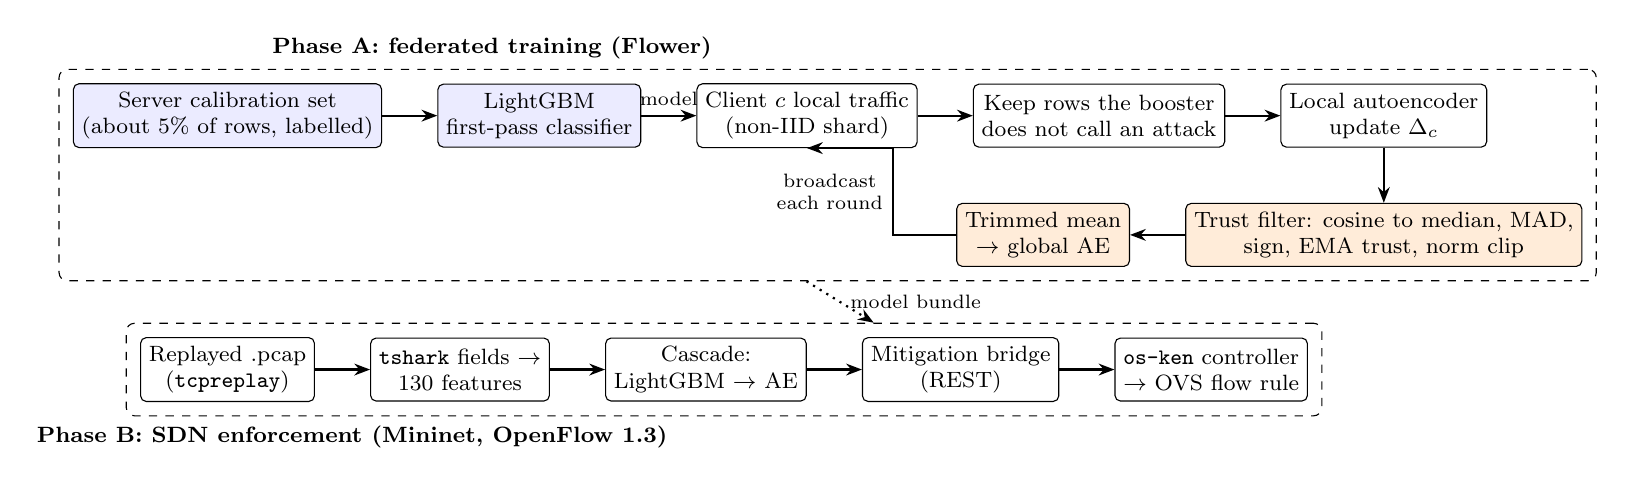
\begin{tikzpicture}[
  node distance=5mm and 7mm,
  box/.style={draw, rounded corners=2pt, align=center, font=\footnotesize, minimum height=8mm, inner sep=3pt, fill=white},
  grp/.style={draw, dashed, rounded corners=3pt, inner sep=5pt},
  arr/.style={-{Stealth[length=2mm]}, thick}]
  % Phase A
  \node[box, fill=blue!8] (cal) {Server calibration set\\(about 5\% of rows, labelled)};
  \node[box, fill=blue!8, right=of cal] (lgb) {LightGBM\\first-pass classifier};
  \node[box, right=of lgb] (cli) {Client $c$ local traffic\\(non-IID shard)};
  \node[box, right=of cli] (keep) {Keep rows the booster\\does not call an attack};
  \node[box, right=of keep] (ae) {Local autoencoder\\update $\Delta_c$};
  \node[box, fill=orange!15, below=7mm of ae] (tf) {Trust filter: cosine to median, MAD,\\sign, EMA trust, norm clip};
  \node[box, fill=orange!15, left=of tf] (tm) {Trimmed mean\\$\rightarrow$ global AE};
  \draw[arr] (cal) -- (lgb);
  \draw[arr] (lgb) -- node[above, font=\scriptsize]{model} (cli);
  \draw[arr] (cli) -- (keep);
  \draw[arr] (keep) -- (ae);
  \draw[arr] (ae) -- (tf);
  \draw[arr] (tf) -- (tm);
  \draw[arr] (tm.west) -- ++(-8mm,0) |- node[pos=0.25, left, font=\scriptsize, align=center]{broadcast\\each round} (cli.south);
  \begin{scope}[on background layer]
    \node[grp, fit=(cal)(lgb)(cli)(keep)(ae)(tf)(tm), label={[font=\footnotesize\bfseries]above left:Phase A: federated training (Flower)}] (pa) {};
  \end{scope}
  % Phase B
  \node[box, below=24mm of cal] (pcap) {Replayed .pcap\\(\texttt{tcpreplay})};
  \node[box, right=of pcap] (feat) {\texttt{tshark} fields $\rightarrow$\\130 features};
  \node[box, right=of feat] (casc) {Cascade:\\LightGBM $\rightarrow$ AE};
  \node[box, right=of casc] (bridge) {Mitigation bridge\\(REST)};
  \node[box, right=of bridge] (ctl) {\texttt{os-ken} controller\\$\rightarrow$ OVS flow rule};
  \draw[arr] (pcap) -- (feat);
  \draw[arr] (feat) -- (casc);
  \draw[arr] (casc) -- (bridge);
  \draw[arr] (bridge) -- (ctl);
  \begin{scope}[on background layer]
    \node[grp, fit=(pcap)(feat)(casc)(bridge)(ctl), label={[font=\footnotesize\bfseries]below left:Phase B: SDN enforcement (Mininet, OpenFlow 1.3)}] (pb) {};
  \end{scope}
  \draw[arr, dotted] ([xshift=95mm]pa.south west) -- node[right, font=\scriptsize]{model bundle} ([xshift=95mm]pb.north west);
\end{tikzpicture}
\end{adjustbox}
\caption{FL-IDS architecture. Phase~A trains the autoencoder federatedly on traffic the boosting stage passes, with a trust filter in front of aggregation. Phase~B loads the resulting bundle and enforces its verdicts as OpenFlow rules.}
\label{fig:arch}
\end{figure*}

The federation has a server and $n$ clients. Each client stands for one site and holds only that site's traffic. Client data are non-IID. The server is trusted, and it holds a small labelled calibration set (Section~\ref{sec:booster}). A fraction $f$ of clients is malicious. A malicious client receives the global model like any other, trains on its own data, and then sends the server an arbitrary update. It may also misreport its number of training examples, which matters for example-weighted rules such as FedAvg. We evaluate two concrete attackers: a sign-flipping client, and a white-box client that knows the filter's rules and shapes its update to pass them (Section~\ref{sec:attackers}). Data-poisoning clients that send honestly computed updates on manipulated local data are outside what an update-level filter can detect; we discuss them in Section~\ref{sec:discussion}.

\subsection{Boosting stage}
\label{sec:booster}
The first stage is a LightGBM multiclass classifier over all 15 labels. Its training labels come from a server-held calibration set of about 5\% of all rows, chosen as whole connections, class by class (Section~\ref{sec:splits}). Part of this set is held back to score each version of the booster: a fifth by configuration, 20 to 28\% in practice because whole connections are taken. The booster weights each class by $\sqrt{N_{\max}/N_c}$, where $N_c$ is the class's training count, so that rare classes count for more without the instability of full inverse-frequency weights. We chose server-held labels over client-held labels because a supervised model needs labels, and IoT sites in practice rarely have analyst-labelled attack traffic. The cost is that this one component is centrally trained (Section~\ref{sec:discussion}). The server trains the classifier before round~1, so clients never filter with an untrained model. In each round, the serialised model (about 9 to 10~MB) travels to the clients inside the round's fit configuration. It is not averaged like the autoencoder; every client runs the same copy locally and caches its filtering result until the model changes.

The boosting stage reads raw feature values. The autoencoder reads per-client normalised values (Section~\ref{sec:ae}). We separated the two after finding that per-client normalisation destroys a shared tree model. Under strong label skew, a client's own scaler can shift a feature by orders of magnitude, so the split thresholds learned on the calibration set no longer apply. In an early test, the same held-out rows passed through a heavily skewed client's scaler were classified almost entirely wrongly.

\textit{Incremental update.} Every three rounds, each client that passed the trust filter in that round surfaces up to 50 rows its autoencoder flagged, with labels confirmed by an analyst. False alarms come back labelled Normal. The server continues training the booster on the calibration set plus all alerts so far (50 more boosting rounds, via LightGBM's initial-model option). If the alerts contain a class the booster has never seen, the server retrains it from scratch, because continued training cannot learn a new class: its predicted probability is near $10^{-14}$, the softmax Hessian for it is near zero, and the minimum-Hessian constraint then blocks every split. This mechanism relaxes the rule that raw traffic never leaves a client. Up to 50 confirmed alert rows per surviving client per update round are sent to the server. We report it as a design trade-off.

\subsection{Client autoencoder}
\label{sec:ae}
Each client trains a dense autoencoder with layers $130\!\to\!32\!\to\!16\!\to\!8\!\to\!16\!\to\!32\!\to\!130$, ReLU between layers and a linear output. It has 9,834 parameters, of which 9,600 are weights and 234 are biases. Training minimises mean squared reconstruction error with Adam~\cite{kingma2015} (learning rate $10^{-3}$, batch size 64, five local epochs per round). A client trains only on the local rows that the current boosting model passes to the second stage: rows predicted Normal, or predicted as an attack with probability below the cascade threshold. The autoencoder therefore models traffic that the supervised stage considers benign or is unsure about.

Inputs are z-scored with each client's own scaler. Global normalisation would leak cross-client distribution statistics and remove the heterogeneity we want to test. We clip z-scores at $\pm10$. Counter-like fields such as \texttt{udp.stream} and \texttt{tcp.seq} can barely vary inside one client's shard. Unclipped, ordinary rows from another part of the capture can then land thousands of standard deviations out and dominate that client's reconstruction error.

Each client calibrates its anomaly threshold $\theta_c$ as the 97th percentile of reconstruction error on a held-out benign validation slice of its own data. It recomputes the threshold every round, because the global model changes every round. By construction, about 3\% of a client's benign validation traffic lies above its threshold. A client whose shard has no benign validation rows gets $\theta_c=\infty$, so its autoencoder never flags. With each update, a client also returns a 50-bin histogram of its reconstruction errors over $[0,10]$ for monitoring.

\subsection{Cascade decision rule}
Evaluation, the dashboard and the SDN bridge all use one implementation of the cascade. For a row $x$ at client $c$, let $\hat y$ be the booster's predicted class and $\hat p$ its probability, and let $e(x)$ be the autoencoder's reconstruction error on the client-normalised row. With confidence threshold $\gamma=0.7$,
\begin{equation}
\mathrm{output}(x)=
\begin{cases}
(\hat y,\hat p) & \text{if } \hat y\neq\text{Normal and } \hat p\ge\gamma,\\
\bigl(\text{anomalous},\ \mathrm{clip}_{[0,1]}\bigl(e(x)/\theta_c-1\bigr)\bigr) & \text{else if } e(x)>\theta_c,\\
(\text{benign},\cdot) & \text{otherwise.}
\end{cases}
\label{eq:cascade}
\end{equation}
The second stage outputs \emph{anomalous}, not an attack type. A reconstruction error can say that a row does not look like benign traffic, but not what attack it belongs to.

\subsection{Trust filter and aggregation}
\label{sec:filter}
Let $w_t$ be the global autoencoder parameters sent out at the start of round $t$, and $w_i$ the parameters client $i$ returns. The filter works on deltas $\Delta_i=w_i-w_t$. Raw weights are dominated by the shared global model, so the cosine similarity between any two clients' raw weights is close to 1 whatever their behaviour. As a reference direction the server uses the coordinate-wise median $r=\mathrm{med}(\Delta_1,\dots,\Delta_n)$, and for each client it computes $s_i=\cos(\Delta_i,r)$. Client $i$ is excluded from the round if any of three conditions holds:
\begin{enumerate}
  \item \textbf{MAD outlier:} $s_i<m-3d$, where $m$ is the median of the round's similarities and $d$ their median absolute deviation~\cite{leys2013};
  \item \textbf{opposes consensus:} $s_i<0$;
  \item \textbf{low trust:} $\tau_i<0.5$ after this round's update, where $\tau_i\leftarrow\alpha\,(s_i+1)/2+(1-\alpha)\tau_i$ with $\alpha=0.3$ and $\tau_i=1$ initially.
\end{enumerate}

\begin{algorithm}[t]
\caption{One round of trust-filtered aggregation}
\label{alg:filter}
\begin{algorithmic}[1]
\Require global weights $w_t$; client weights $w_1,\dots,w_n$; trust scores $\tau$
\State $\Delta_i\gets w_i-w_t$ for all $i$
\State $r\gets$ coordinate-wise median of $\{\Delta_i\}$
\State $s_i\gets\cos(\Delta_i,r)$;\ $m\gets\mathrm{med}(s)$;\ $d\gets\mathrm{med}(|s-m|)$
\State $\tau_i\gets 0.3\,(s_i+1)/2+0.7\,\tau_i$
\State $S\gets\{i: s_i\ge m-3d\ \wedge\ s_i\ge 0\ \wedge\ \tau_i\ge 0.5\}$
\If{$S=\emptyset$} \State \Return $w_t$ \EndIf
\State $c\gets 2\cdot\mathrm{med}_j\,\lVert\Delta_j\rVert$
\State $\tilde\Delta_i\gets\Delta_i\cdot\min(1,\,c/\lVert\Delta_i\rVert)$ for $i\in S$
\State $k\gets\lfloor 0.15\,|S|\rfloor$
\State \Return $w_t+\mathrm{TrimmedMean}_k(\{\tilde\Delta_i\}_{i\in S})$
\end{algorithmic}
\end{algorithm}

Each rule addresses a specific failure. The MAD threshold is relative to the round: under heavy non-IID skew, honest clients can have low similarity to the median, and a fixed cosine cutoff would either reject them or admit attackers depending on the split. MAD alone is not enough, though. In an earlier version that used only this rule, honest heterogeneity widened the MAD band until attackers with negative similarity fell inside it. The sign rule is the same boundary FLTrust uses when it gives updates with negative cosine to the reference zero weight~\cite{cao2021fltrust}. It is a fixed point, the sign, rather than a tuned value. The trust rule makes a client's history count, the role temporal analysis plays in~\cite{li2021spatial}.

Cosine similarity ignores magnitude. The filter also clips each surviving delta to $2\times$ the round's median norm, $\tilde\Delta_i=\Delta_i\min\bigl(1,\,2\,\mathrm{med}_j\lVert\Delta_j\rVert/\lVert\Delta_i\rVert\bigr)$. The clipped survivors are combined by a coordinate-wise trimmed mean~\cite{yin2018} that drops $\lfloor 0.15|S|\rfloor$ values from each side, where $S$ is the survivor set. The result is added to $w_t$. If no client survives, the round's aggregation is skipped. Example counts reported by clients are ignored throughout. Algorithm~\ref{alg:filter} summarises one round. The filter keeps no state other than the trust scores, and it never sees data. The aggregation runs inside a custom Flower strategy that subclasses FedAvg. Its fit-configuration step records $w_t$ for the delta computation and attaches the current boosting model. Its aggregation step runs Algorithm~\ref{alg:filter} and passes the surviving clients' alerts to the boosting update.

\subsection{SDN enforcement}
\label{sec:sdn}
Phase~B rebuilds every model from the Phase~A bundle, never from the current configuration. The bundle holds the booster, the final autoencoder weights, each client's scaler and threshold, the z-score clip, the cascade settings, held-out metrics and provenance (seed, commit, time). Phase~B rejects a bundle whose thresholds, recomputed from the saved weights, do not match the clients' final-round values.

Mininet~\cite{lantz2010} brings up one Open vSwitch~\cite{pfaff2015} switch and one host per FL client. Host $h_{i+1}$ is scored with client $i$'s scaler and threshold. The switch is controlled by an OpenFlow~1.3 controller we built on \texttt{os-ken}, the maintained OpenStack fork of Ryu. A real Edge-IIoTset capture is replayed from a host with \texttt{tcpreplay}. \texttt{tshark} extracts the authors' fields with the corrections of Section~\ref{sec:defects}, and the same code that built the training matrix derives the 130 features, including the connection features, from the capture. To check for training/serving skew~\cite{breck2019}, we compared the live rows from the Backdoor capture with that capture's training rows: 99.8\% of the 24,914 live rows are identical to a training row across all 130 features. The cascade then classifies every row.

The rows are reduced to one verdict per device. If any row is non-benign, the verdict is the most frequent non-benign label, its confidence is the mean confidence of those rows, and its stage is the stage that made most of those calls. Otherwise the verdict is benign. A REST bridge receives \{device, label, confidence, stage\} and asks the controller for an action. Confidence of at least 0.85 installs a drop rule on the device's source address. Confidence of at least 0.5 attaches an OpenFlow meter that rate-limits it. Anything lower is left to monitoring. The controller reads switch state back through OpenFlow multipart statistics requests, so what it reports is what \texttt{ovs-ofctl dump-flows} shows. The topology is written so a switch port can bridge to a physical or virtual NIC, which would put an external device's traffic under the same controller. That path is designed but not yet built.

\section{Experimental Setup}
\label{sec:setup}
\subsection{Splits by connection}
\label{sec:splits}
Every split in the federated system keeps each connection whole. The server's calibration set takes whole connections, class by class, until it holds about 5\% of each class's rows. The remaining pool, all of it, is divided among the clients with a Dirichlet label-skew partition~\cite{hsu2019} with concentration $\alpha=0.3$. For each class, a Dirichlet draw gives each client a target share, and connections in random order go to whichever client is furthest below its target. Each client then sets aside about 15\% of its rows as a test slice and about 15\% of its remaining benign rows as a benign validation slice for threshold calibration, again by whole connections. The rest is its training data. No connection appears in more than one of these sets.

A class with fewer than 20 connections cannot be split this way. Only MITM is affected: its 406 rows form a single connection, so all of it goes to the server's calibration set. The booster learns MITM, but no client holds MITM rows and no test slice contains any. MITM is evaluated only by the zero-day experiment and the Phase~B replay. Twenty-four connections (655 rows) carry two labels and are split by label.

Table~\ref{tab:sizes} gives the resulting sizes. The seed changes the calibration set, the partition and the model initialisation. Because whole connections are chosen, the server set varies between 100,024 and 100,181 rows across seeds. Of it, 71,853 to 79,866 rows train the booster and the rest score it. The clients together hold about 1.89 million rows, and their test slices hold 283,090 to 295,566 rows. Strong skew leaves some clients without benign validation rows. They get an infinite threshold, so their autoencoder never flags.

\begin{table}[t]
\centering
\caption{Data sizes and Phase~A wall time of the six real runs. ``Server train'' and ``held back'' are the two parts of the calibration set; ``no benign val.'' counts clients with no benign validation rows.}
\label{tab:sizes}
\small
\setlength{\tabcolsep}{3pt}
\begin{adjustbox}{max width=\linewidth}
\begin{tabular}{rrrrrrrr}
\toprule
Clients & Seed & Server train & Held back & Client rows & Test rows & No ben.\ val. & Phase A (s) \\
\midrule
10 & 42 & 79,866 & 20,315 & 1,885,587 & 288,416 & 1 & 1844 \\
10 & 43 & 72,803 & 27,221 & 1,885,744 & 283,090 & 0 & 1397 \\
10 & 44 & 71,853 & 28,242 & 1,885,673 & 288,366 & 2 & 1754 \\
20 & 42 & 79,866 & 20,315 & 1,885,587 & 283,427 & 3 & 1260 \\
20 & 43 & 72,803 & 27,221 & 1,885,744 & 292,222 & 2 & 1063 \\
20 & 44 & 71,853 & 28,242 & 1,885,673 & 295,566 & 0 & 1225 \\
\bottomrule
\end{tabular}
\end{adjustbox}
\end{table}

\subsection{Real runs and in-process experiments}
Six real runs train the system as a deployed federation would: a Flower server and one operating-system process per client, 20 rounds, no attackers, with 10 and 20 clients and seeds 42, 43 and 44. Each run saves a model bundle, which we score on the clients' test slices. The 10-client, seed-42 bundle also drives Phase~B.

The ablation, poisoning sweep, zero-day, stealth-attacker, pruning and clip experiments take separate training jobs that drive the same client, attacker and aggregation code in one process instead of over gRPC, with 10 clients and 20 rounds on the same full-pool splits. The sweep, ablation, zero-day, stealth-attacker, pruning-during-training and clip experiments all run with three seeds. Pruning after training is a single run on the seed-42 bundle.

\subsection{Attackers}
\label{sec:attackers}
A \emph{sign-flipping} client trains honestly for the round and then returns $w_t-5(w_i-w_t)$, its true delta negated and amplified five times. It reports the largest example count of any client, so that FedAvg, which weights updates by reported counts, gives it as much weight as possible. The trust filter and trimmed mean ignore counts. At a malicious fraction $f$, $\mathrm{round}(fn)$ clients are drawn without replacement using the run's seed.

A \emph{stealth} client is a white-box attacker that knows the filter's cosine rule and norm clip. It estimates the consensus direction as the last aggregate update it can observe (this round's global weights minus last round's). Its update keeps a cosine of 0.1 to that direction and spends the rest of its norm budget, 1.5 times its honest norm and so below the $2\times$ clip, on the negative of the part of its honest update that is orthogonal to the consensus. In round~1 it has no estimate and behaves honestly. This is one adaptive strategy, not a bound over all of them.

We do not use label flipping or input corruption as test attackers. The autoencoder never sees labels, and corrupted inputs mostly make a client look like one more heterogeneous client, so neither would test an update-level defence.

\subsection{Variants}
Every variant uses the same data, partition and seed.
\begin{itemize}
  \item \texttt{full\_pipeline}: the trust filter and trimmed mean, the boosting pre-filter for autoencoder training, and the cascade of Eq.~(\ref{eq:cascade}).
  \item \texttt{plain\_fedavg}: as above, with FedAvg in place of the filter and trimmed mean.
  \item \texttt{trimmed\_mean\_only}: the trimmed mean without the trust filter.
  \item \texttt{autoencoder\_only}: the autoencoder trained on all local rows with no boosting pre-filter. Detection is the autoencoder alone.
  \item \texttt{boosting\_only}: the cascade rule without the second stage, and no FL. A row counts as detected when the booster labels it an attack with probability at least $\gamma$.
\end{itemize}

\subsection{Metrics}
About 72\% of the rows are benign, so accuracy mostly tracks the benign false-positive rate, and it even rises when a poisoned autoencoder stops flagging anything. We report the following instead.
\begin{itemize}
  \item \textbf{Attack macro-recall:} the share of attack rows flagged (labelled with any attack type, or anomalous), averaged over the attack classes present in the test slices with equal weight. In the federated tests this is 13 classes, because MITM has no test rows.
  \item \textbf{Attack micro-recall:} the same, pooled over all attack rows.
  \item \textbf{Packet false-alarm rate:} the share of benign test rows flagged.
  \item \textbf{Connection false-alarm rate:} the share of benign test connections in which at least half the rows are flagged. We also report the median client's packet rate, and the share of all false-alarm packets that come from the ten largest benign connections.
  \item \textbf{Autoencoder-alone macro-recall:} attack macro-recall when the autoencoder flags every row by itself. It isolates the federated component, whose damage under poisoning the cascade otherwise hides.
  \item \textbf{Attacker survival:} the share of attacker-rounds in which an attacker's update passed the filter into aggregation.
\end{itemize}
The test set is the union of the clients' test slices, and each row is scored with its own client's scaler and threshold, as in deployment.

\textit{Zero-day protocol.} For each of the 14 attack classes in turn, we remove that class from the calibration set and from every client's data before partitioning, so it is absent even from the scaler statistics. We train, then score every row of the held-out class (from 406 rows for MITM to 121,567 for DDoS\_UDP) as unseen traffic. Each row is assigned to a random client and scored with that client's scaler and threshold. A row counts as detected if the cascade flags it in any way. We report the detection rate per class and its mean over the 14 classes, for the classifier alone, the autoencoder alone and the cascade.

\textit{Pruning.} We prune the autoencoder by global weight magnitude, zeroing the smallest fraction of weight-matrix entries and keeping the biases. During training, the server re-prunes the global model after every aggregation, with the target sparsity ramped linearly over the first ten rounds. After training, we prune the final model of the 10-client, seed-42 real run and recalibrate the thresholds. Reported sizes assume a sparse encoding (float32 values plus int32 indices). Clients still train and send dense updates, so this shrinks the stored model, not the per-round communication.

\subsection{Standalone classifier studies}
Three studies evaluate the first-stage classifier alone and centrally.
\begin{itemize}
  \item \textbf{Feature study.} LightGBM on all rows at the natural class distribution, for each step from the 91 base features to the full 130. Each feature set gets its own deduplication. Each is evaluated on two 80/20 splits: a split stratified by class over individual rows, and the first fold of a five-fold stratified group split with the connection as the group, so that no connection has rows on both sides. We treat the second as the main result. MITM lies wholly on one side of it and is left out of its macro F1. LightGBM uses 63 leaves, learning rate 0.1, feature and bagging fractions of 0.8, leaf regularisation, early stopping (patience 50) on 10\% of the training rows and, in the final configuration, the class weights of Section~\ref{sec:booster}. It ran with four threads, so it is reproducible only to within thread-scheduling noise.
  \item \textbf{Time-ordered split.} The same final configuration, with each class's earliest 80\% of connections in training and its latest 20\% in test, for seeds 42 to 44. CSV row order is capture order within each class. The CSV records time of day without a date, so this orders by row position, not by a verified clock.
  \item \textbf{Model selection.} LightGBM against other classifiers on the same split. Section~\ref{sec:models} describes this study in full.
\end{itemize}

\begin{table}[t]
\centering
\caption{Hyperparameters of the federated system (from the run configuration files).}
\label{tab:hyper}
\small
\begin{adjustbox}{max width=\linewidth}
\begin{tabular}{lll}
\toprule
Component & Parameter & Value \\
\midrule
Data & clients $n$ / Dirichlet $\alpha$ / seeds & 10 or 20 / 0.3 / 42, 43, 44 \\
 & test / benign-validation fraction & 0.15 / 0.15 \\
 & z-score clip / min.\ connections per class & $\pm10$ / 20 \\
LightGBM & calibration fraction / held-back share & 0.05 / 0.2 \\
 & boosting rounds / learning rate / leaves & 300 / 0.05 / 31 \\
 & min.\ leaf Hessian / L2 / class weights & 1.0 / 1.0 / square root \\
 & update every / extra rounds / alerts per client & 3 rounds / 50 / 50 \\
Autoencoder & layers & 130--32--16--8--16--32--130 \\
 & optimiser / lr / batch / local epochs & Adam / $10^{-3}$ / 64 / 5 \\
 & anomaly percentile & 97 \\
Cascade & confidence threshold $\gamma$ & 0.7 \\
FL & rounds & 20 \\
Trust filter & MAD multiplier / min.\ cosine / min.\ trust & 3.0 / 0.0 / 0.5 \\
 & EMA $\alpha$ / norm-clip multiplier / trim per side & 0.3 / 2.0 / 0.15 \\
Attackers & sign-flip amplification / claimed count & 5 / largest client \\
 & stealth cosine target / norm multiplier & 0.1 / 1.5 \\
SDN & block / rate-limit confidence & 0.85 / 0.5 \\
\bottomrule
\end{tabular}
\end{adjustbox}
\end{table}

\subsection{Hyperparameters and implementation}
Table~\ref{tab:hyper} lists the settings. The cascade threshold, 97th percentile, trim fraction, norm-clip multiplier and SDN thresholds come from the project specification, set in an earlier prototype, and were not tuned on the test data. The LightGBM regularisation was added because training without it overfitted the small calibration set, and its benign false-alarm rate swung widely when a small share of calibration rows changed. In the pipeline, LightGBM runs single-threaded in deterministic mode, because multi-threaded histogram construction did not reproduce exactly across identical runs.

The system is written in Python with PyTorch~\cite{paszke2019} 2.14, Flower~\cite{beutel2020} 1.38, LightGBM 4.7 and \texttt{os-ken} 4.2, with Mininet and Open vSwitch for the network and \texttt{tcpreplay} and \texttt{tshark} for traffic. All experiments ran in an Ubuntu virtual machine with 20 virtual CPUs and 48~GB of memory. A real 20-client run needs about 28~GB, so real runs were never run alongside other jobs. The test suite (247 passed, one skipped) passes in this environment.

\section{System Results}
\label{sec:results}
\subsection{Real multi-process runs}
\label{sec:real}
Table~\ref{tab:real} reports the six real runs on the clients' test slices, 283,090 to 295,566 rows per run, with no attackers. Known attacks are detected almost completely. The cascade's micro-recall is 0.9956 to 0.9989 and its macro-recall over the 13 attack classes present is 0.9939 to 0.9981. The booster alone reaches 0.9954 to 0.9981 micro-recall, so on known attacks the autoencoder adds between 0.0002 and 0.0008. The bootstrap booster, scored on the held-back part of the calibration set, reaches 0.9947 to 0.9980 accuracy and 0.9609 to 0.9871 macro F1 (Table~\ref{tab:filterhonest}).

\begin{table*}[t]
\centering
\caption{Six real multi-process runs (20 rounds, no attackers), scored on the clients' test slices. Recall columns: cascade macro- and micro-recall, booster-alone micro-recall, autoencoder-alone macro-recall. False-alarm columns: all benign test packets, the median client's packets, benign connections with half or more of their packets flagged, and the share of false-alarm packets that come from the ten largest benign connections.}
\label{tab:real}
\small
\begin{adjustbox}{max width=\linewidth}
\begin{tabular}{rrcccccccc}
\toprule
 & & \multicolumn{4}{c}{Recall on known attacks} & \multicolumn{4}{c}{False alarms} \\
\cmidrule(lr){3-6}\cmidrule(lr){7-10}
Clients & Seed & Macro & Micro & Booster & AE alone & Packets & Median client & Connections & Top-10 share \\
\midrule
10 & 42 & 0.9958 & 0.9974 & 0.9970 & 0.461 & 0.1275 & 0.0286 & 0.0034 & 0.94 \\
10 & 43 & 0.9947 & 0.9978 & 0.9971 & 0.463 & 0.0884 & 0.0313 & 0.0074 & 0.80 \\
10 & 44 & 0.9939 & 0.9956 & 0.9954 & 0.220 & 0.0248 & 0.0293 & 0.0039 & 0.89 \\
20 & 42 & 0.9981 & 0.9989 & 0.9981 & 0.718 & 0.0588 & 0.0322 & 0.0104 & 0.52 \\
20 & 43 & 0.9970 & 0.9980 & 0.9974 & 0.619 & 0.1628 & 0.0307 & 0.0076 & 0.87 \\
20 & 44 & 0.9972 & 0.9978 & 0.9972 & 0.709 & 0.1089 & 0.0296 & 0.0081 & 0.90 \\
\bottomrule
\end{tabular}
\end{adjustbox}
\end{table*}

\textit{False alarms.} The packet false-alarm rate varies from 2.5\% to 16.3\% across the six runs, and nearly all of it comes from the second stage: the booster alone flags 0.012\% to 0.046\% of benign packets. The packet rate is a poor summary, because a few very long benign connections dominate it. In the 10-client, seed-42 run, client 9 holds a benign connection of 11,764 packets that the autoencoder flags in full. In five of the six runs, 80 to 94\% of all false-alarm packets come from the ten largest benign connections, and 52\% in the sixth. The median client's packet rate is 2.9 to 3.2\% in every run, close to the 3\% the 97th-percentile threshold implies. Counted per connection, 0.34 to 1.04\% of the 10,765 to 12,519 benign test connections have half or more of their packets flagged (Fig.~\ref{fig:fa}). An operator who acts on connections would see roughly one false alarm per hundred benign connections. One who acts on packets would see many more, concentrated in a handful of long-lived sessions.

\begin{figure}[t]
\centering
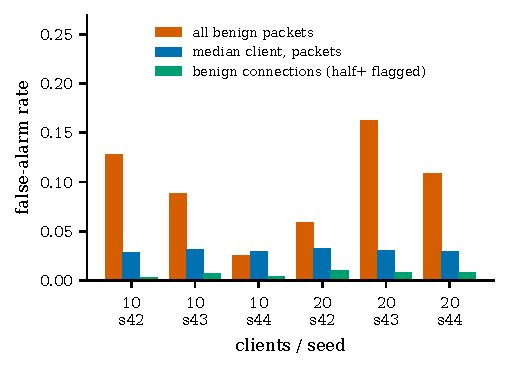
\includegraphics[width=\columnwidth]{figs/fig_fa.pdf}
\caption{False-alarm rate of the six real runs, counted three ways.}
\label{fig:fa}
\end{figure}

\textit{The autoencoder on its own.} Alone, the autoencoder detects between 22\% and 72\% of attack packets. It is weaker with 10 clients (0.220 to 0.463) than with 20 (0.619 to 0.718), and it varies strongly with the seed. Table~\ref{tab:perclass} shows why it still matters little for known attacks. Per class, the booster detects 0.984 to 1.000 and the cascade 0.987 to 1.000, while the autoencoder alone ranges from 0.037 on Backdoor to 0.939 on DDoS\_TCP. Its value lies in attack types the booster has never seen (Section~\ref{sec:zeroday}).

\textit{The filter with no attackers.} Even with no attacker present, the filter excluded 6 to 12 of 200 client-rounds in the 10-client runs and 12 to 19 of 400 in the 20-client runs (Table~\ref{tab:filterhonest}). Every exclusion but one was a MAD outlier. These are honest clients whose non-IID updates differ from the median, which is the confound discussed in Section~\ref{sec:discussion}.

\begin{table}[t]
\centering
\caption{Bootstrap booster scored on the held-back calibration rows, and honest client-rounds the trust filter excluded during each real run (no attackers present).}
\label{tab:filterhonest}
\small
\begin{adjustbox}{max width=\linewidth}
\begin{tabular}{rrccc}
\toprule
Clients & Seed & Accuracy & Macro F1 & Client-rounds excluded \\
\midrule
10 & 42 & 0.9947 & 0.9808 & 12 / 200 \\
10 & 43 & 0.9971 & 0.9609 & 6 / 200 \\
10 & 44 & 0.9980 & 0.9871 & 7 / 200 \\
20 & 42 & 0.9947 & 0.9808 & 19 / 400 \\
20 & 43 & 0.9971 & 0.9609 & 12 / 400 \\
20 & 44 & 0.9980 & 0.9871 & 12 / 400 \\
\bottomrule
\end{tabular}
\end{adjustbox}
\end{table}

\begin{table}[t]
\centering
\caption{Recall per attack type by stage, 10 clients, seed 42, with the range of cascade recall over all six real runs. MITM has no test rows (Section~\ref{sec:splits}).}
\label{tab:perclass}
\small
\setlength{\tabcolsep}{3pt}
\begin{adjustbox}{max width=\linewidth}
\begin{tabular}{lrcccc}
\toprule
Class & Test rows & Booster & AE alone & Cascade & Cascade, six runs \\
\midrule
Backdoor & 2,263 & 0.9885 & 0.037 & 0.9929 & 0.9729--0.9983 \\
DDoS\_HTTP & 6,915 & 0.9899 & 0.481 & 0.9899 & 0.9856--0.9963 \\
DDoS\_ICMP & 9,520 & 1.0000 & 0.317 & 1.0000 & 0.9997--1.0000 \\
DDoS\_TCP & 6,717 & 1.0000 & 0.939 & 1.0000 & 1.0000--1.0000 \\
DDoS\_UDP & 17,755 & 0.9999 & 0.306 & 1.0000 & 1.0000--1.0000 \\
Fingerprinting & 129 & 0.9845 & 0.070 & 0.9922 & 0.9730--1.0000 \\
Password & 7,795 & 0.9913 & 0.252 & 0.9914 & 0.9875--0.9963 \\
Port\_Scanning & 2,929 & 1.0000 & 0.684 & 1.0000 & 0.9982--1.0000 \\
Ransomware & 691 & 0.9841 & 0.488 & 0.9870 & 0.9847--0.9975 \\
SQL\_injection & 7,228 & 0.9990 & 0.894 & 0.9996 & 0.9976--1.0000 \\
Uploading & 5,567 & 0.9998 & 0.549 & 0.9998 & 0.9995--1.0000 \\
Vuln.\ scanner & 7,216 & 0.9946 & 0.501 & 0.9961 & 0.9925--0.9996 \\
XSS & 2,274 & 0.9960 & 0.471 & 0.9969 & 0.9893--0.9991 \\
\bottomrule
\end{tabular}
\end{adjustbox}
\end{table}

Phase~A took 1,063 to 1,844~s for 20 rounds (Table~\ref{tab:sizes}); 871 to 1,633~s of that is federated training, 16~s the calibration split, bootstrap classifier and client partition, and 156 to 191~s evaluation. Some runs shared the machine with other jobs, so these times are upper bounds.

\subsection{Ablation and poisoning sweep}
The in-process experiments reproduce the real runs closely. With no attackers, in-process attack macro-recall is 0.996, 0.996 and 0.994 for the three seeds, against 0.9958, 0.9947 and 0.9939 in the 10-client real runs. Table~\ref{tab:ablation} compares the five variants with three sign-flipping clients out of ten, and Table~\ref{tab:sweep} with Fig.~\ref{fig:poison} follows the full pipeline from 0\% to 50\% attackers.

\begin{table*}[t]
\centering
\caption{Ablation with 30\% sign-flipping clients, 10 clients, 20 rounds. Each cell lists seeds 42 / 43 / 44. The full-pipeline row is the sweep's 30\% point.}
\label{tab:ablation}
\small
\begin{adjustbox}{max width=\linewidth}
\begin{tabular}{llll}
\toprule
Variant & Attack macro-recall & AE-alone macro-recall & Benign FPR (packets) \\
\midrule
full\_pipeline & 0.995 / 0.997 / 0.995 & 0.490 / 0.373 / 0.245 & 0.1112 / 0.0653 / 0.0075 \\
plain\_fedavg & 0.992 / 0.994 / 0.990 & 0.013 / 0.002 / 0.092 & 0.0947 / 0.0301 / 0.0301 \\
trimmed\_mean\_only & 0.995 / 0.995 / 0.993 & 0.205 / 0.000 / 0.025 & 0.1070 / 0.0261 / 0.0299 \\
autoencoder\_only & 0.105 / 0.073 / 0.051 & 0.105 / 0.073 / 0.051 & 0.0473 / 0.0411 / 0.0445 \\
boosting\_only & 0.990 / 0.989 / 0.982 & -- & 0.0001 / 0.0001 / 0.0003 \\
\bottomrule
\end{tabular}
\end{adjustbox}
\end{table*}

\begin{table}[t]
\centering
\caption{Poisoning sweep, full pipeline, 10 clients, 20 rounds. Seeds 42 / 43 / 44.}
\label{tab:sweep}
\small
\setlength{\tabcolsep}{3pt}
\begin{adjustbox}{max width=\linewidth}
\begin{tabular}{rllll}
\toprule
Attackers & Attack macro-recall & AE-alone recall & Survival & Benign FPR \\
\midrule
0\% & 0.996 / 0.996 / 0.994 & 0.457 / 0.492 / 0.221 & -- & 0.118 / 0.041 / 0.035 \\
20\% & 0.995 / 0.996 / 0.994 & 0.466 / 0.483 / 0.258 & 0.30 / 0.40 / 0.23 & 0.105 / 0.094 / 0.037 \\
30\% & 0.995 / 0.997 / 0.995 & 0.490 / 0.373 / 0.245 & 0.50 / 0.55 / 0.62 & 0.111 / 0.065 / 0.008 \\
40\% & 0.994 / 0.994 / 0.992 & 0.297 / 0.139 / 0.074 & 0.60 / 0.64 / 0.61 & 0.091 / 0.038 / 0.043 \\
50\% & 0.995 / 0.990 / 0.985 & 0.249 / 0.000 / 0.000 & 0.64 / 1.00 / 0.99 & 0.115 / 0.052 / 0.030 \\
\bottomrule
\end{tabular}
\end{adjustbox}
\end{table}

\begin{figure*}[t]
\centering
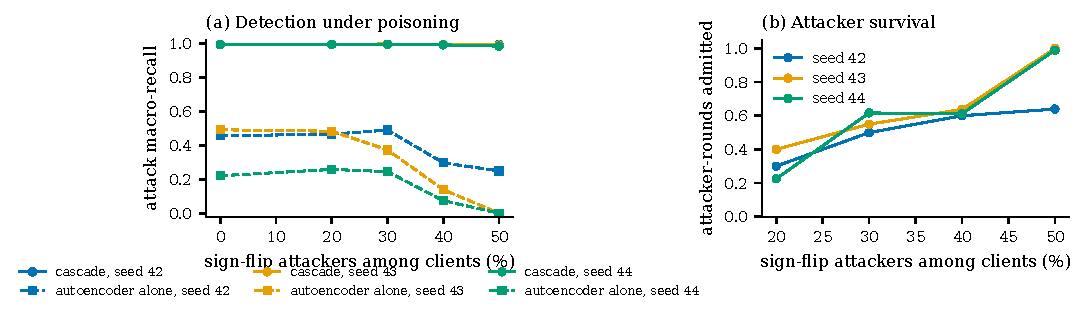
\includegraphics[width=\textwidth]{figs/fig_poison.pdf}
\caption{Full pipeline under increasing shares of sign-flipping clients, three seeds. (a) Known-attack macro-recall of the cascade (solid) and macro-recall of the autoencoder alone (dashed). (b) Share of attacker-rounds in which an attacker passed the filter.}
\label{fig:poison}
\end{figure*}

\textit{Known attacks are safe from poisoning.} Every variant that includes the booster keeps attack macro-recall between 0.982 and 0.997, and the full pipeline stays between 0.985 and 0.997 at every attacker fraction up to 50\%. The booster is trained on the server, so poisoned updates cannot reach it. Reported on its own, this number would hide what happens to the federated part.

\textit{Robust aggregation protects the autoencoder at 30\%.} The full pipeline's autoencoder detects 0.490, 0.373 and 0.245 at 30\% attackers, against 0.457, 0.492 and 0.221 with no attackers. Under plain FedAvg it detects 0.013, 0.002 and 0.092, and under the trimmed mean without the filter 0.205, 0.000 and 0.025. The trimmed mean alone fails because, with ten clients and a 15\% trim, it removes one update from each side, and three colluding attackers outnumber that. This is the expected breakdown of the rule~\cite{yin2018}. The margin over plain FedAvg is smallest at seed 44, where the autoencoder was weak to begin with.

\textit{The filter admits many attackers at this scale.} Attackers reached aggregation in 23 to 40\% of their rounds at 20\% attackers and in 50 to 62\% at 30\%. The autoencoder still holds at 30\%. Our reading, which we have not tested separately, is that the filter removes enough attackers for the stages after it to cope: at a survival of 0.50 to 0.62, about 1.5 to 1.9 of the three attackers pass in an average round, and the norm clip and one-per-side trim bound what they can do. At 40\% the autoencoder degrades to 0.297, 0.139 and 0.074. At 50\%, attackers are admitted in 64\%, 100\% and 99\% of their rounds and the autoencoder fails in two of three seeds. Once half the clients attack, the coordinate-wise median moves toward their direction, and any defence that takes the median as its consensus fails there.

\textit{The pre-filter matters.} Trained on all local traffic instead of boosting-filtered traffic, the autoencoder detects only 0.105, 0.073 and 0.051. Filtering out traffic the booster already recognises as attack leaves the autoencoder a much cleaner picture of benign behaviour.

\textit{The cascade's gain on known attacks is small and its false alarms vary.} Compared with boosting alone at 30\% attackers, the full pipeline gains 0.005 to 0.014 in macro-recall. Its packet false-alarm rate ranges from 0.75\% to 11.1\% across seeds, against at most 0.03\% for the booster alone. The spread follows the long-connection effect described above.

\subsection{Unseen attack types}
\label{sec:zeroday}
Fig.~\ref{fig:zeroday} and Table~\ref{tab:zeroday} report the leave-one-class-out experiment with no attackers. In all 42 cases (14 classes, three seeds), the cascade detects at least as much of the held-out class as the better of its two stages alone. Its mean detection rate over the 14 classes is 0.910, 0.944 and 0.895 for the three seeds, against 0.735, 0.757 and 0.723 for the classifier alone and 0.681, 0.728 and 0.590 for the autoencoder alone. The cost is a mean benign packet false-alarm rate of 0.079 to 0.104 across the held-out runs.

The held-out classes fall into three groups.

\textit{The classifier finds them anyway, under the wrong name.} DDoS\_ICMP, Fingerprinting, Port\_Scanning and Ransomware are detected at 0.982 or more by the classifier alone, because it maps each to a behaviourally similar class it knows. Held-out Port\_Scanning is labelled Fingerprinting in 99 to 100\% of rows, and held-out Ransomware is labelled Backdoor in 97 to 99\%. The detection counts, but an operator would see a confident alert with the wrong attack type.

\textit{Mostly the autoencoder finds them.} For DDoS\_UDP and MITM, the classifier alone detects 0.021 to 0.416 and 0.005 to 0.200. The cascade detects 0.803 to 0.905 and 0.751 to 1.000, almost all from the second stage. MITM is a single connection of 406 rows, so its numbers swing widely between seeds.

\textit{Hard for both, or seed-dependent.} Uploading is the weakest class in every seed (cascade 0.527 to 0.665). The classifier lets 70 to 80\% of it through as benign or with low confidence, and the autoencoder finds it only partly unusual. Backdoor (0.743 at seed 42, 0.998 otherwise) and Vulnerability\_scanner (0.859 at seed 44, 0.992 otherwise) depend on the seed, in both cases through the classifier alone, which detects 0.486 and 0.335 in the weak seed against more than 0.89 in the others.

\begin{figure}[t]
\centering
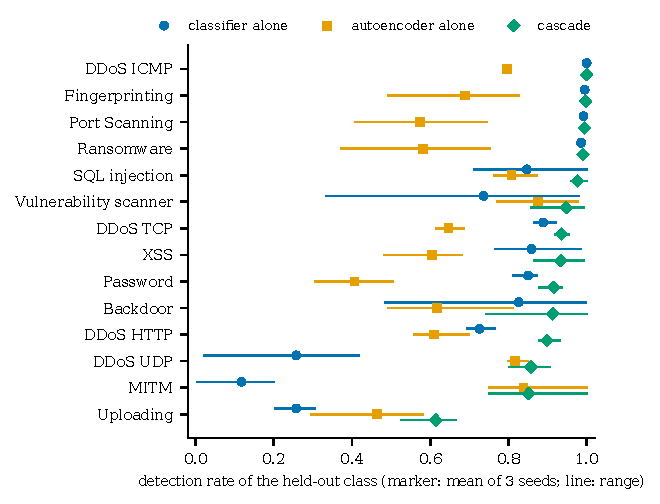
\includegraphics[width=\columnwidth]{figs/fig_zeroday.pdf}
\caption{Detection of each attack type when it is withheld from all training data, by stage. Classes are ordered by the cascade's mean detection rate.}
\label{fig:zeroday}
\end{figure}

\begin{table*}[t]
\centering
\caption{Leave-one-class-out detection, 10 clients, 0\% attackers, every row of the held-out class scored. Seeds 42 / 43 / 44.}
\label{tab:zeroday}
\small
\begin{adjustbox}{max width=\linewidth}
\begin{tabular}{lrlll}
\toprule
Held-out class & Rows & Classifier alone & Autoencoder alone & Cascade \\
\midrule
Backdoor & 24,167 & 0.486 / 0.996 / 0.997 & 0.493 / 0.550 / 0.810 & 0.743 / 0.998 / 0.998 \\
DDoS\_HTTP & 49,768 & 0.695 / 0.764 / 0.719 & 0.572 / 0.698 / 0.560 & 0.879 / 0.932 / 0.885 \\
DDoS\_ICMP & 68,758 & 1.000 / 1.000 / 0.999 & 0.786 / 0.802 / 0.800 & 1.000 / 1.000 / 1.000 \\
DDoS\_TCP & 50,062 & 0.865 / 0.921 / 0.879 & 0.640 / 0.686 / 0.615 & 0.933 / 0.953 / 0.921 \\
DDoS\_UDP & 121,567 & 0.416 / 0.021 / 0.334 & 0.849 / 0.799 / 0.799 & 0.905 / 0.803 / 0.866 \\
Fingerprinting & 872 & 0.995 / 0.994 / 0.994 & 0.826 / 0.747 / 0.492 & 0.998 / 0.998 / 0.997 \\
MITM & 406 & 0.148 / 0.200 / 0.005 & 0.764 / 1.000 / 0.751 & 0.803 / 1.000 / 0.751 \\
Password & 50,033 & 0.872 / 0.865 / 0.813 & 0.505 / 0.407 / 0.307 & 0.932 / 0.935 / 0.880 \\
Port\_Scanning & 20,213 & 0.998 / 0.988 / 0.989 & 0.570 / 0.745 / 0.409 & 0.999 / 0.993 / 0.992 \\
Ransomware & 9,885 & 0.984 / 0.990 / 0.982 & 0.621 / 0.753 / 0.374 & 0.990 / 0.994 / 0.988 \\
SQL\_injection & 50,981 & 0.828 / 0.713 / 0.999 & 0.764 / 0.871 / 0.787 & 0.961 / 0.970 / 0.999 \\
Uploading & 37,243 & 0.204 / 0.266 / 0.304 & 0.581 / 0.512 / 0.295 & 0.665 / 0.652 / 0.527 \\
Vuln.\ scanner & 50,044 & 0.980 / 0.894 / 0.335 & 0.880 / 0.976 / 0.772 & 0.992 / 0.993 / 0.859 \\
XSS & 15,172 & 0.823 / 0.986 / 0.767 & 0.680 / 0.650 / 0.483 & 0.943 / 0.991 / 0.867 \\
\midrule
Mean over 14 classes & & 0.735 / 0.757 / 0.723 & 0.681 / 0.728 / 0.590 & 0.910 / 0.944 / 0.895 \\
\bottomrule
\end{tabular}
\end{adjustbox}
\end{table*}

\subsection{An adaptive attacker}
\label{sec:adaptive}
Table~\ref{tab:stealth} compares the stealth attacker with the sign-flipping one over three seeds. The filter catches the stealth attacker less often: it survives 0.60 to 0.95 of its rounds at 20\% attackers, 0.68 to 0.83 at 30\% and 0.80 to 0.85 at 40\%, against 0.23 to 0.40, 0.50 to 0.62 and 0.60 to 0.64 for sign-flipping. The extra survival does not buy much more damage. The autoencoder-alone recall under stealth attackers is 0.220 to 0.588 at 20\%, 0.316 to 0.427 at 30\% and 0.045 to 0.334 at 40\%; under sign-flipping it is 0.258 to 0.483, 0.245 to 0.490 and 0.074 to 0.297. Eight of the nine seed and fraction pairs differ by less than 0.1 between the two attackers, and the stealth attacker leaves the lower recall in five of the nine. Known-attack recall stays at 0.9908 or above in every run. We did not measure zero-day detection under either attacker, so the harm to the part of the system that matters most for unseen attacks is still open.

\begin{table*}[t]
\centering
\caption{Stealth versus sign-flipping attackers, 10 clients, 20 rounds. Each cell lists seeds 42 / 43 / 44.}
\label{tab:stealth}
\small
\begin{adjustbox}{max width=\linewidth}
\begin{tabular}{lccccc}
\toprule
 & \multicolumn{2}{c}{Attacker survival} & \multicolumn{2}{c}{AE-alone recall} & Known-attack recall \\
\cmidrule(lr){2-3}\cmidrule(lr){4-5}\cmidrule(lr){6-6}
Attackers & Sign-flip & Stealth & Sign-flip & Stealth & Stealth \\
\midrule
20\% & 0.30 / 0.40 / 0.23 & 0.60 / 0.70 / 0.95 & 0.466 / 0.483 / 0.258 & 0.454 / 0.588 / 0.220 & 0.9956 / 0.9961 / 0.9942 \\
30\% & 0.50 / 0.55 / 0.62 & 0.73 / 0.68 / 0.83 & 0.490 / 0.373 / 0.245 & 0.427 / 0.329 / 0.316 & 0.9961 / 0.9956 / 0.9953 \\
40\% & 0.60 / 0.64 / 0.61 & 0.80 / 0.80 / 0.85 & 0.297 / 0.139 / 0.074 & 0.334 / 0.160 / 0.045 & 0.9949 / 0.9939 / 0.9908 \\
\bottomrule
\end{tabular}
\end{adjustbox}
\end{table*}

\subsection{Pruning and the z-score clip}
\label{sec:prune}
Table~\ref{tab:prunefl} reports pruning during federated training, over three seeds with no attackers. The autoencoder learns around the zeros up to a point. Its recall falls from 0.457, 0.492 and 0.221 at no pruning to 0.439, 0.376 and 0.210 at 50\% sparsity, then to 0.350, 0.369 and 0.168 at 70\%, 0.338, 0.209 and 0.145 at 80\%, and 0.198, 0.059 and 0.092 at 90\%. The cascade's known-attack recall stays at 0.993 or above in every run, because the booster carries it.

\begin{table}[t]
\centering
\caption{Pruning during federated training (server re-prunes each round), 10 clients, no attackers. Seeds 42 / 43 / 44.}
\label{tab:prunefl}
\small
\begin{adjustbox}{max width=\linewidth}
\begin{tabular}{rrlll}
\toprule
Sparsity & Non-zero weights & AE-alone recall & Cascade macro-recall & Benign FPR \\
\midrule
0\% & 9,600 & 0.457 / 0.492 / 0.221 & 0.996 / 0.996 / 0.994 & 0.118 / 0.041 / 0.035 \\
50\% & 4,800 & 0.439 / 0.376 / 0.210 & 0.995 / 0.993 / 0.994 & 0.140 / 0.040 / 0.030 \\
70\% & 2,880 & 0.350 / 0.369 / 0.168 & 0.993 / 0.996 / 0.994 & 0.120 / 0.078 / 0.024 \\
80\% & 1,920 & 0.338 / 0.209 / 0.145 & 0.993 / 0.994 / 0.994 & 0.145 / 0.058 / 0.025 \\
90\% & 960 & 0.198 / 0.059 / 0.092 & 0.993 / 0.994 / 0.993 & 0.115 / 0.026 / 0.025 \\
\bottomrule
\end{tabular}
\end{adjustbox}
\end{table}

Pruning after training is one run (the 10-client, seed-42 bundle, thresholds recalibrated; Table~\ref{tab:prunepost}) and is much worse at the same sparsity. Recall falls from 0.461 to 0.375 at 50\% and to 0.098 at 70\%, and the AUROC of the reconstruction error falls from 0.892 to 0.495, no better than chance. The 9,834-parameter autoencoder is already small, and a sparse encoding only saves space beyond 50\% sparsity, where the model starts to lose recall. Pruning buys little here.

\begin{table}[t]
\centering
\caption{Pruning after training (10-client, seed-42 real-run bundle, thresholds recalibrated; one run). Sparse size is relative to the dense model.}
\label{tab:prunepost}
\small
\setlength{\tabcolsep}{3pt}
\begin{adjustbox}{max width=\linewidth}
\begin{tabular}{rrcccccc}
\toprule
Sparsity & Non-zero & Sparse size & AE recall & AE AUROC & Cascade macro-recall & Benign FPR \\
\midrule
0\% & 9,600 & 1.98 & 0.461 & 0.892 & 0.996 & 0.1275 \\
50\% & 4,800 & 1.00 & 0.375 & 0.788 & 0.995 & 0.0814 \\
70\% & 2,880 & 0.61 & 0.098 & 0.495 & 0.994 & 0.0418 \\
80\% & 1,920 & 0.41 & 0.110 & 0.451 & 0.995 & 0.0692 \\
90\% & 960 & 0.22 & 0.092 & 0.461 & 0.995 & 0.0607 \\
95\% & 480 & 0.12 & 0.093 & 0.460 & 0.995 & 0.0781 \\
98\% & 192 & 0.06 & 0.094 & 0.467 & 0.995 & 0.0783 \\
\bottomrule
\end{tabular}
\end{adjustbox}
\end{table}

The z-score clip matters more than a single run suggested. Without it, the final benign validation loss of the autoencoder is 0.242 at seed 42, against 0.129 with the clip. At seeds 43 and 44 the loss without the clip is 117.8 and 102.8, against 0.057 and 0.264 with it. In two of three seeds, then, training without the clip fails outright, because rows from another part of the capture land thousands of standard deviations from a client's statistics and dominate its reconstruction error.

\subsection{Live replay through the SDN}
\label{sec:replay}
Phase~B loaded the 10-client, seed-42 bundle and replayed each of the 14 attack captures from host $h_1$ (Table~\ref{tab:phaseb}). Every replay ended in a block decision, and the rule \texttt{priority=100,ip,nw\_src=10.0.0.1 actions=drop} was read back from the switch each time. Twelve of the 14 captures were given the right attack type, all by the booster. The MITM capture was called Ransomware, with only 542 of its 1,229 packets flagged. The OS-fingerprinting capture was called DDoS\_ICMP. Both are still blocked. The replays took 8 to 268~s, the longest for the 3.2-million-packet DDoS\_UDP capture.

Two facts limit what this shows. The captures are the dataset's own, so their rows are in the training data and the replay is a demonstration of the pipeline, not a held-out test. And the drop rule appears only after \texttt{tshark} has processed the whole capture: when it was read back, it had matched no packets, because the replay had already finished. Phase~B is batch classification of a capture, not inline blocking.

\begin{table*}[t]
\centering
\caption{Phase~B on every attack capture (10-client, seed-42 bundle). Confidence is the mean over the non-benign packets of the chosen label. All verdicts came from the booster.}
\label{tab:phaseb}
\small
\begin{adjustbox}{max width=\linewidth}
\begin{tabular}{llcrcr}
\toprule
Capture & Classified as & Confidence & Packets flagged & Action & Wall time (s) \\
\midrule
Backdoor attack & Backdoor & 0.997 & 24,543 / 24,914 & block & 12 \\
DDoS HTTP flood & DDoS\_HTTP & 0.966 & 119,748 / 229,142 & block & 29 \\
DDoS ICMP flood & DDoS\_ICMP & 1.000 & 2,914,156 / 2,914,356 & block & 232 \\
DDoS TCP SYN flood & DDoS\_TCP & 0.999 & 2,020,023 / 2,020,152 & block & 211 \\
DDoS UDP flood & DDoS\_UDP & 0.999 & 2,899,758 / 3,215,732 & block & 268 \\
MITM ARP spoofing + DNS & \textit{Ransomware} & 0.991 & 542 / 1,229 & block & 8 \\
OS fingerprinting & \textit{DDoS\_ICMP} & 0.980 & 1,134 / 1,176 & block & 9 \\
Password attacks & Password & 0.957 & 919,469 / 1,053,893 & block & 130 \\
Port scanning & Port\_Scanning & 0.999 & 22,495 / 23,329 & block & 12 \\
Ransomware & Ransomware & 0.994 & 10,620 / 11,030 & block & 11 \\
SQL injection & SQL\_injection & 1.000 & 51,097 / 51,228 & block & 17 \\
Uploading & Uploading & 0.999 & 37,592 / 37,644 & block & 15 \\
XSS & XSS & 0.999 & 15,677 / 16,215 & block & 12 \\
Vulnerability scanner & Vulnerability\_scanner & 0.996 & 262,922 / 265,827 & block & 60 \\
\bottomrule
\end{tabular}
\end{adjustbox}
\end{table*}

\subsection{Features for the first stage}
\label{sec:featstudy}
Table~\ref{tab:feat} follows LightGBM from the 91 base features to the full 130 on all rows. On the connection-grouped split, macro F1 rises from 0.889 to 0.924 with the service port, stays level with the content features, and jumps to 0.981 with the connection features. Content features add little on their own, because few packets carry content, but they feed the connection aggregates. Class weights bring the final configuration to 0.983, with accuracy 0.997. The ambiguity ceiling rises from 0.969 to 0.9997 macro recall, and the share of rows whose feature vector also occurs with another label falls from 2.31\% to 0.01\%. The random and grouped splits differ by at most 0.007 in macro F1 for every feature set, so neither feature set was relying on memorised connections.

\begin{table}[t]
\centering
\caption{LightGBM on all rows, seed 42, from the base features to the final 130. Random = rows split at random; grouped = connections held out. The ceiling is the best accuracy and macro recall any classifier on that feature set could reach.}
\label{tab:feat}
\small
\setlength{\tabcolsep}{2.5pt}
\begin{adjustbox}{max width=\linewidth}
\begin{tabular}{lrrcccccc}
\toprule
 & & & \multicolumn{2}{c}{Random} & \multicolumn{2}{c}{Grouped} & \multicolumn{2}{c}{Ceiling} \\
\cmidrule(lr){4-5}\cmidrule(lr){6-7}\cmidrule(lr){8-9}
Features & Count & Rows & Acc. & F1 & Acc. & F1 & Acc. & Rec. \\
\midrule
Base (authors' recipe) & 91 & 1,909,719 & 0.9638 & 0.8868 & 0.9637 & 0.8892 & 0.9875 & 0.9692 \\
+ service port & 92 & 1,909,980 & 0.9802 & 0.9245 & 0.9803 & 0.9236 & 0.9985 & 0.9940 \\
+ content & 110 & 1,909,980 & 0.9802 & 0.9268 & 0.9802 & 0.9232 & 0.9985 & 0.9940 \\
+ connection & 130 & 1,985,768 & 0.9977 & 0.9879 & 0.9975 & 0.9808 & 0.9999 & 0.9997 \\
+ class weights & 130 & 1,985,768 & 0.9976 & 0.9867 & 0.9972 & 0.9828 & 0.9999 & 0.9997 \\
\bottomrule
\end{tabular}
\end{adjustbox}
\end{table}

Fig.~\ref{fig:f1} shows where the gain comes from. The application-layer classes that the base features could not separate (Fingerprinting, Uploading, DDoS\_HTTP, SQL\_injection, Password and XSS) rise from 0.68--0.85 F1 to 0.93--1.00. Of the 1,113 remaining errors at seed 42, 54\% are Password and DDoS\_HTTP confused with each other, both HTTP requests to the same server, and 14\% are Ransomware and Backdoor confused with each other (Fig.~\ref{fig:cm}).

\begin{figure}[t]
\centering
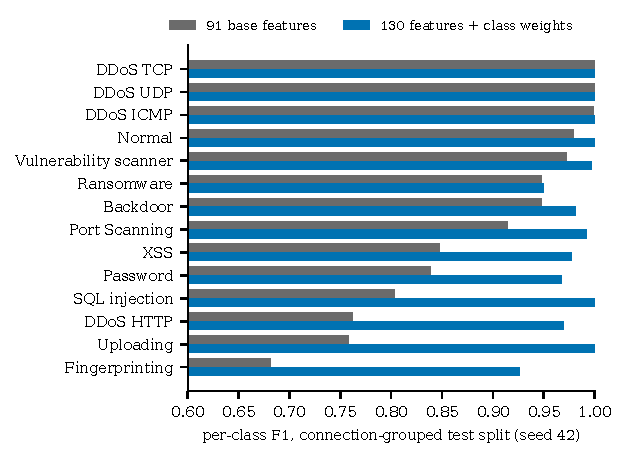
\includegraphics[width=\columnwidth]{figs/fig_f1.pdf}
\caption{Per-class F1 of LightGBM with the 91 base features and with the final 130 features and class weights, connection-grouped split, seed 42. MITM cannot be scored on this split.}
\label{fig:f1}
\end{figure}

\begin{figure}[t]
\centering
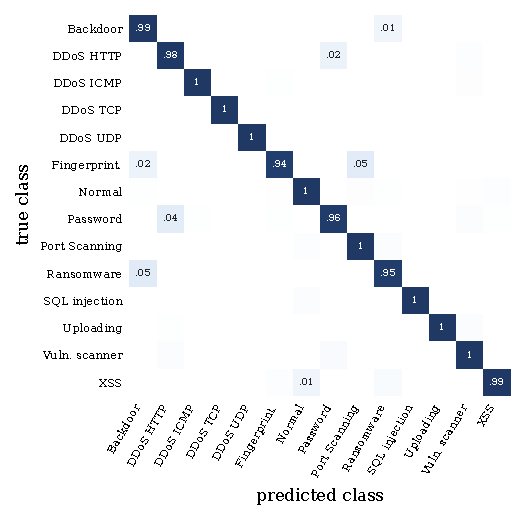
\includegraphics[width=\columnwidth]{figs/fig_cm.pdf}
\caption{Confusion matrix of the final classifier (130 features, class weights), connection-grouped test split, seed 42, row-normalised. Shading is stretched (square-root scale) so that small errors are visible.}
\label{fig:cm}
\end{figure}

Table~\ref{tab:seeds} repeats the final configuration over three seeds. Grouped macro F1 is 0.983, 0.984 and 0.985. Without class weights it swings from 0.981 to 0.952, because Fingerprinting, with few connections, varies widely. The same configuration trained on only 5\% of the rows, the size of the calibration set, reaches 0.997 accuracy and 0.979 macro F1 on the same grouped test set, against 0.962 and 0.881 for the base features under the same restriction. So the bootstrap booster in the federated system is not much weaker for training on the server's small set.

Two of the added features owe part of their value to the testbed. Benign traffic in Edge-IIoTset is MQTT and VNC and never HTTP, so a service port of 80 alone hints at an attack. In a network with benign web traffic, that feature would separate much less. The keyword groups were chosen with the dataset's attack families in mind, which makes them closer to signatures than to general behaviour.

\textit{Time-ordered split.} Training on each class's earlier connections and testing on its later ones gives 0.994 accuracy and 0.912 to 0.913 macro F1 over three seeds (Table~\ref{tab:seeds}). The lower macro F1 is mostly an artifact. MITM is one connection, so this split puts it entirely in the test side, where its recall of 0 enters the mean of 15 classes. Without MITM, the seed-42 macro F1 would be about 0.978. The real losses are on Backdoor (recall 0.947 to 0.962, against 0.989 on the grouped split) and DDoS\_HTTP (0.912 to 0.925, against 0.980).

\begin{table}[t]
\centering
\caption{Final classifier configuration across seeds: random split, grouped split, grouped split without class weights, and time-ordered split.}
\label{tab:seeds}
\small
\setlength{\tabcolsep}{3pt}
\begin{adjustbox}{max width=\linewidth}
\begin{tabular}{rcccccc}
\toprule
 & Random & \multicolumn{2}{c}{Grouped} & Grouped, no weights & \multicolumn{2}{c}{Time-ordered} \\
\cmidrule(lr){2-2}\cmidrule(lr){3-4}\cmidrule(lr){5-5}\cmidrule(lr){6-7}
Seed & F1 & Acc. & F1 & F1 & Acc. & F1 \\
\midrule
42 & 0.9867 & 0.9972 & 0.9828 & 0.9808 & 0.9942 & 0.9133 \\
43 & 0.9868 & 0.9971 & 0.9835 & 0.9560 & 0.9943 & 0.9122 \\
44 & 0.9866 & 0.9970 & 0.9851 & 0.9521 & 0.9941 & 0.9129 \\
\bottomrule
\end{tabular}
\end{adjustbox}
\end{table}

\subsection{Communication, training time and decision time}
The autoencoder's 9,834 float32 parameters cost $2\times9{,}834\times4=78{,}672$ bytes per client per round, downlink plus uplink: 786,720 bytes per round for 10 clients and 15,734,400 over 20 rounds. That figure leaves out the booster, which the server sends to every client every round. Its serialised file is 8.9 to 10.4~MB across the six runs, so one client's copy alone is more than ten times a whole round of autoencoder traffic for ten clients. Sending it only when its version changes, at most every third round, is a simple saving we have not implemented.

We timed the cascade on the saved 10-client, seed-42 bundle, one CPU thread of the VM's Intel Xeon, with 3,000 held-out test packets timed one call each and one batch of 200,000. The classifier alone takes a median 0.372~ms per packet (95th percentile 0.440), the autoencoder alone 0.060~ms (0.094), and both stages 0.642~ms (0.706). In batch mode the cascade handles 3,760 packets per second, 265.9~$\mu$s per packet, almost all of it in the booster (the autoencoder alone takes 5.5~$\mu$s). These are model times only: they exclude reading a capture, \texttt{tshark} feature extraction and the switch, and they come from one bundle on one machine, so we claim no confidence interval.

\section{Model Selection Study}
\label{sec:models}
The first stage of the cascade is LightGBM, and this section tests that choice. The study ran in three stages. Two earlier stages on other datasets compared classical machine learning with deep learning, and a wider stage surveyed about 50 classical models on the same two datasets. A new comparison on Edge-IIoTset then used the split, features and metric of the rest of this paper. The earlier stages are public repositories of the same project; every number below is read from their result files.

\subsection{Earlier stages on MQTTset and DataSense}
Stage~1 compared eight supervised classifiers on MQTTset~\cite{vaccari2020}: random forest, logistic regression, gradient boosting, k-nearest neighbours, naive Bayes, an MLP, a 1D-CNN and a GRU, plus a one-class autoencoder trained on benign traffic. An RBF SVM, an LSTM and a vanilla RNN were added to the table. Stage~2 repeated the method on DataSense~\cite{firouzi2025}, the 2025 sensor-based IIoT benchmark from the Canadian Institute for Cybersecurity. Table~\ref{tab:prior} lists the results. Neither dataset gave a clear winner between the two families. On MQTTset, k-nearest neighbours had the highest macro F1 (0.819), ahead of the MLP (0.777), the GRU (0.768) and gradient boosting (0.724). On DataSense, the MLP (0.895) and gradient boosting (0.893) were level and the random forest followed at 0.884. The recurrent networks without sequence input were poor on both (LSTM 0.243 and vanilla RNN 0.095 macro F1 on DataSense). When the same CNN and GRU were retrained on windows of eight packets per flow, accuracy on MQTTset rose to 0.999, but that test measures a different task on a different sample and we do not compare it with the flat-feature models.

\begin{table}[t]
\centering
\caption{Earlier stages: classical and neural classifiers on MQTTset and DataSense, ordered by macro F1 within each dataset. MQTTset: 231,646 training and 99,290 test rows, 33 features. DataSense: 31,538 training and 13,517 test rows, 109 features. $^\dagger$ trained on a 40,000-row subsample because the full fit did not finish.}
\label{tab:prior}
\small
\begin{adjustbox}{max width=\linewidth}
\begin{tabular}{lccc}
\toprule
Model & Accuracy & Macro F1 & Train (s) \\
\midrule
\textit{MQTTset} & & & \\
\quad K-Nearest Neighbors & 0.9136 & 0.8188 & 0.0 \\
\quad MLP & 0.8513 & 0.7768 & 42.8 \\
\quad GRU & 0.8496 & 0.7681 & 122.7 \\
\quad Gradient Boosting & 0.8883 & 0.7235 & 4.4 \\
\quad Random Forest & 0.8856 & 0.7157 & 1.6 \\
\quad LSTM & 0.8286 & 0.6560 & 276.8 \\
\quad Logistic Regression & 0.6520 & 0.6305 & 9.7 \\
\quad 1D-CNN & 0.7312 & 0.6207 & 99.9 \\
\quad SVM (RBF)$^\dagger$ & 0.6467 & 0.5679 & 23.4 \\
\quad RNN & 0.8202 & 0.5038 & 212.9 \\
\quad Naive Bayes & 0.7946 & 0.4759 & 0.1 \\
\textit{DataSense} & & & \\
\quad MLP & 0.9448 & 0.8948 & 63.9 \\
\quad Gradient Boosting & 0.9516 & 0.8931 & 7.0 \\
\quad Random Forest & 0.9418 & 0.8842 & 0.8 \\
\quad 1D-CNN & 0.9244 & 0.8596 & 39.8 \\
\quad K-Nearest Neighbors & 0.9129 & 0.8452 & 0.0 \\
\quad SVM (RBF) & 0.8841 & 0.7667 & 22.2 \\
\quad GRU & 0.8672 & 0.7470 & 126.5 \\
\quad Logistic Regression & 0.8568 & 0.7357 & 1.3 \\
\quad Naive Bayes & 0.4655 & 0.4344 & 0.0 \\
\quad LSTM & 0.6228 & 0.2434 & 94.4 \\
\quad RNN & 0.6072 & 0.0945 & 103.0 \\
\bottomrule
\end{tabular}
\end{adjustbox}

\end{table}

Stage~3 widened the classical side. It trained about 50 scikit-learn-compatible classifiers on both datasets, covering linear models, naive Bayes, single trees, bagged trees, boosting (XGBoost, LightGBM, CatBoost, HistGradientBoosting and others), kernel and instance-based learners, interpretable models and ensembles. It ranked them by a composite of quality (macro F1, weighted F1 and F1 on the rarest class) and cost (inference time and training time), with weights of 0.7 for quality and 0.3 for cost. Stage~3 reuses the split of the first two stages (a model in both gives the same macro F1; k-nearest neighbours with $k=5$ scores 0.8188 on MQTTset in both), but it sub-sampled some slow models. Table~\ref{tab:top} lists the ten highest composite scores. Gradient-boosting implementations take the first five places, XGBoost first, with LightGBM fourth. This ranking is the reason boosting went forward. It has two limits: the cost weights were our own choice, and both datasets are far smaller and simpler than Edge-IIoTset.

\begin{table}[t]
\centering
\caption{Stage~3: ten best of 50 classical models by average composite score over MQTTset and DataSense (quality weight 0.7, cost weight 0.3).}
\label{tab:top}
\small
\begin{adjustbox}{max width=\linewidth}
\begin{tabular}{llccc}
\toprule
Model & Family & F1 MQTTset & F1 DataSense & Composite \\
\midrule
XGBoost (DART) & boosting & 0.8371 & 0.9618 & 99.9 \\
XGBoost & boosting & 0.8371 & 0.9618 & 99.9 \\
Hist Gradient Boosting & boosting & 0.8350 & 0.9585 & 99.5 \\
LightGBM & boosting & 0.8370 & 0.9614 & 99.5 \\
CatBoost & boosting & 0.8339 & 0.9523 & 99.2 \\
Gradient Boosting (sklearn) & boosting & 0.8334 & 0.9553 & 96.5 \\
K-Nearest Neighbors (k=15, distance-weighted) & instance & 0.8274 & 0.8487 & 92.4 \\
Explainable Boosting Machine & interpretable & 0.8284 & 0.9555 & 91.9 \\
K-Nearest Neighbors (k=5) & instance & 0.8188 & 0.8452 & 91.8 \\
Voting Classifier (soft) & meta & 0.7618 & 0.9210 & 90.5 \\
\bottomrule
\end{tabular}
\end{adjustbox}

\end{table}

\subsection{Comparison on Edge-IIoTset}
\label{sec:zoo}
\textit{Protocol.} The new comparison uses the 130-feature matrix and the connection-grouped split of Section~\ref{sec:featstudy} (seed 42): 397,073 test rows, none from a connection seen in training. Every model trains on the same class-capped stratified sample of 500,000 training rows, because slow learners cannot be run on all 1.43 million, and is scored on the full test split. Hyperparameters were chosen on a separate validation sample of 60,000 rows and never on the test rows. Each model had a small grid (for example tree depth, number of leaves, regularisation strength or $k$); the grid and the chosen value are stored with the results. Models that accept class weights use the same square-root weights as the system, and the neural networks use them in the loss. The RBF SVM was trained on a 40,000-row subsample and the GRU on 150,000 rows, for the same feasibility reason. Metrics are accuracy, macro F1 over the classes present in the test split, benign false-positive rate, training time on 16 CPU threads and prediction time per row.

\begin{table*}[t]
\centering
\caption{Edge-IIoTset, 130 features, connection-grouped test split (397,073 rows, seed 42): 15 classifiers trained on the same 500,000-row sample, ordered by macro F1. Train and predict times are wall-clock on 16 CPU threads, one job at a time. Values marked $^\ddagger$ come from a separate run of that model alone on the machine.}
\label{tab:zoo}
\small
\begin{adjustbox}{max width=\linewidth}
\begin{tabular}{llccccrr}
\toprule
Model & Family & Acc. & Macro F1 & Weighted F1 & Benign FPR & Train (s) & Predict ($\mu$s/row) \\
\midrule
Random forest & bagging trees & 0.9970 & 0.9848 & 0.9970 & 0.0010 & 13 & 3.8 \\
HistGradientBoosting & boosting & 0.9970 & 0.9838 & 0.9970 & 0.0012 & 39$^\ddagger$ & 15.5$^\ddagger$ \\
XGBoost & boosting & 0.9971 & 0.9834 & 0.9972 & 0.0010 & 30 & 1.2 \\
Decision tree & single tree & 0.9967 & 0.9828 & 0.9968 & 0.0010 & 7 & 0.1 \\
CatBoost & boosting & 0.9970 & 0.9813 & 0.9970 & 0.0011 & 315 & 0.7 \\
LightGBM & boosting & 0.9971 & 0.9805 & 0.9971 & 0.0010 & 8 & 1.3 \\
Extra trees & bagging trees & 0.9968 & 0.9792 & 0.9968 & 0.0010 & 19 & 3.8 \\
k-nearest neighbours & instance & 0.9956 & 0.9706 & 0.9956 & 0.0012 & 0$^\ddagger$ & 261.3$^\ddagger$ \\
1D-CNN & neural & 0.9953 & 0.9640 & 0.9954 & 0.0016 & 96$^\ddagger$ & 17.6$^\ddagger$ \\
MLP & neural & 0.9959 & 0.9631 & 0.9959 & 0.0015 & 18$^\ddagger$ & 0.2$^\ddagger$ \\
Logistic regression & linear & 0.9937 & 0.9314 & 0.9941 & 0.0016 & 56 & 0.1 \\
GRU (150k train rows) & neural & 0.9857 & 0.9253 & 0.9856 & 0.0038 & 388 & 21.1 \\
RBF SVM (40k train rows) & kernel & 0.9901 & 0.9217 & 0.9905 & 0.0039 & 19$^\ddagger$ & 837.8$^\ddagger$ \\
Linear SVM & linear & 0.9912 & 0.9093 & 0.9925 & 0.0017 & 7 & 0.1 \\
Gaussian naive Bayes & probabilistic & 0.5258 & 0.7115 & 0.6456 & 0.5886 & 0 & 4.4 \\
\bottomrule
\end{tabular}
\end{adjustbox}

\end{table*}

\begin{figure}[t]
\centering
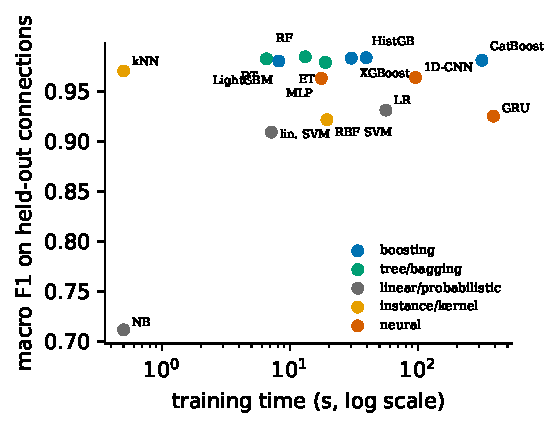
\includegraphics[width=\columnwidth]{figs/fig_zoo.pdf}
\caption{Macro F1 against training time for the 15 classifiers of Table~\ref{tab:zoo}.}
\label{fig:zoo}
\end{figure}

\textit{Results.} Seven tree-based models fill the top of Table~\ref{tab:zoo}, with macro F1 between 0.979 and 0.985: random forest 0.985, HistGradientBoosting 0.984, XGBoost 0.983, a single decision tree 0.983, CatBoost 0.981, LightGBM 0.981 and extra trees 0.979. The spread of 0.006 is the same size as the seed-to-seed spread of one model, since LightGBM on the full training set scores 0.983, 0.984 and 0.985 across the three seeds of Table~\ref{tab:seeds}. We therefore do not rank these seven. k-nearest neighbours follows at 0.971, the 1D-CNN and the MLP at 0.964 and 0.963, logistic regression at 0.931, the RBF SVM on 40,000 rows at 0.922 and the linear SVM at 0.909. Gaussian naive Bayes collapses (0.712, with 59\% of benign rows flagged); it was also among the weakest models in the earlier stages. The GRU, which reads the 130 features as a sequence of 130 steps, reached 0.925 after 20 epochs on 150,000 rows. A first 3-epoch run scored only 0.106, and the 20-epoch validation score was still rising, so we treat the GRU as under-trained and its score as no final value for that architecture. The benign false-positive rate is 0.10 to 0.12\% for every tree model and rises to 0.15 to 0.16\% for the neural networks and logistic regression.

On this feature set the choice among tree models hardly matters: a single decision tree of depth 20 is within 0.002 of the best. That fits the feature study of Section~\ref{sec:featstudy}. Once the connection features make the classes separable (the ambiguity ceiling is 0.9997 macro recall), the model has little left to add. The trees do beat the neural networks, by about 0.02 macro F1, and the linear models by 0.05 or more. Cost separates the families less than accuracy does. The trees train in 7 to 39~s (CatBoost 315~s), the MLP in 18~s, the 1D-CNN in 96~s and the GRU in 388~s. A prediction takes 0.1 to 16~$\mu$s per row for every tree model, 0.2 to 26~$\mu$s for the networks, and 261 and 838~$\mu$s for the two instance-based and kernel models.

\subsection{Boosting on the base features}
\label{sec:basezoo}
The earlier head-to-head of LightGBM and an MLP used the 91 base features and showed a large gap, 0.887 against 0.622 macro F1 on a 500,000-row class-capped sample (Table~\ref{tab:mlp}). The gap was largest on the application-layer attacks that the base features cannot separate. To see how much of it comes from the features rather than the learners, we repeated the comparison above with the 91 base features. Nine of the 15 models were run (the other six were not repeated); Table~\ref{tab:zoobase} gives the results. On the base features the boosting implementations lead clearly: XGBoost 0.875, LightGBM 0.854 and CatBoost 0.852, against 0.807 for the random forest, 0.788 for extra trees and 0.777 for a single decision tree. The MLP (0.596), k-nearest neighbours (0.560) and logistic regression (0.402) are far behind. The MLP's score is close to the 0.622 of the earlier head-to-head, which used a different sample. Adding the 39 service-port, content and connection features raises every model, from $+0.11$ for XGBoost to $+0.53$ for logistic regression, and it closes the gap between boosting and the bagged trees: random forest gains $+0.18$ and reaches the top of Table~\ref{tab:zoo}. The two feature sets give different test rows (381,742 and 397,073, because deduplication differs), so the differences are approximate.

\begin{table}[t]
\centering
\caption{Nine classifiers on the 91 base features and on the 130 features (connection-grouped split, seed 42; 500,000 training rows). The last column is the macro-F1 gain from the 39 added features.}
\label{tab:zoobase}
\small
\begin{adjustbox}{max width=\linewidth}
\begin{tabular}{lcccc}
\toprule
Model & Acc.\ (91) & Macro F1 (91) & Macro F1 (130) & Gain \\
\midrule
XGBoost & 0.9416 & 0.8748 & 0.9834 & +0.1086 \\
LightGBM & 0.9330 & 0.8541 & 0.9805 & +0.1264 \\
CatBoost & 0.9311 & 0.8519 & 0.9813 & +0.1294 \\
Random forest & 0.9104 & 0.8068 & 0.9848 & +0.1780 \\
Extra trees & 0.9056 & 0.7877 & 0.9792 & +0.1914 \\
Decision tree & 0.8912 & 0.7774 & 0.9828 & +0.2054 \\
MLP & 0.8240 & 0.5956 & 0.9631 & +0.3675 \\
k-nearest neighbours & 0.7349 & 0.5603 & 0.9706 & +0.4103 \\
Logistic regression & 0.4781 & 0.4018 & 0.9314 & +0.5296 \\
\bottomrule
\end{tabular}
\end{adjustbox}

\end{table}

So the earlier result and the new one agree. Boosting is the best choice when the features are weak, and its edge over bagged trees disappears when the features are strong.

\begin{table}[t]
\centering
\caption{LightGBM against a dense MLP on the 91 base features, 500,000-row class-capped sample (400,000 training and 100,000 test rows, random split; Normal is about 10\% of the sample). The MLP has hidden layers of 64 and 32 units, dropout 0.1 and 8,271 parameters, trained for 15 epochs.}
\label{tab:mlp}
\small
\begin{tabular}{lcc}
\toprule
 & LightGBM & MLP \\
\midrule
Accuracy & 0.8908 & 0.6779 \\
Macro F1 & 0.8872 & 0.6218 \\
Weighted F1 & 0.8924 & 0.6681 \\
Benign FPR & 0.1599 & 0.5341 \\
Training time (s) & 55.5 & 10.2 \\
Model size & 12.8 MB (300 rounds) & 8,271 parameters \\
\bottomrule
\end{tabular}
\end{table}

In that comparison the gap is largest on XSS (recall 0.761 against 0.072), SQL\_injection (0.767 against 0.213), Fingerprinting (0.579 against 0.000), Port\_Scanning (0.997 against 0.499) and Uploading (0.630 against 0.198), and near zero on the three DDoS floods, which both models classify almost perfectly. The MLP is slightly better on Password and DDoS\_ICMP. The comparison is limited: the MLP is small and was not tuned, the sample uses the unrepaired MITM rows, and its class mix makes the false-alarm rates incomparable with the rest of the paper.

\subsection{Why LightGBM}
Three results favour boosting and one does not. Boosting implementations took the first five places among 50 classical models on two other datasets (stage~3), and on the 91 base features LightGBM beat the MLP by 0.27 macro F1. On the 130 features LightGBM sits inside the top group of tree models, trains in 8~s and produces a model of 9 to 10~MB. It also supports continued training from an existing model, which the incremental update of Section~\ref{sec:booster} needs. What the study does not show is that boosting is the best first stage on the 130 features: random forest, HistGradientBoosting, XGBoost and a single decision tree scored as high or higher in this run. We kept LightGBM because the system was built and evaluated around it before this comparison was run.

\section{Discussion}
\label{sec:discussion}
\subsection{What each part contributes}
Measured separately, the five parts do different jobs. The booster detects almost all known attacks (micro-recall 0.9954 to 0.9981 in the real runs). Because it is trained on the server, poisoned updates cannot reach it. The federated autoencoder adds at most 0.0008 on known attacks and supplies most of the system's benign false alarms. It earns its place on attack types the booster has never seen, where the cascade raises mean detection from 0.723--0.757 to 0.895--0.944, and on classes such as DDoS\_UDP and MITM it is nearly the whole defence. The trust filter, with the norm clip and trimmed mean, keeps the autoencoder usable at 30\% sign-flipping attackers, where plain FedAvg destroys it. SDN enforcement works end to end on all 14 captures, but only as batch classification of a finished capture.

A cascade-level recall therefore says little about whether the federated part works. With 30\% attackers, plain FedAvg keeps 0.990 to 0.994 known-attack macro-recall while its autoencoder detects between 0.2\% and 9.2\% of attack packets. We think evaluations of hybrid federated detectors should report the federated component's own recall and its detection of unseen classes, not only the combined number.

\subsection{False alarms}
The packet false-alarm rate (2.5 to 16.3\%) would make the system unusable if it were the right measure. It is driven by a few very long benign connections. When one of them looks unusual to a client's autoencoder, thousands of packets are flagged at once. Per connection the rate is 0.34 to 1.04\%, and the median client sits near the 3\% the threshold implies. Two changes would address this directly. A device verdict could require a minimum share of flagged packets within a time window, rather than the current rule of any one non-benign packet. And the threshold could be set per connection rather than per packet. Neither is implemented.

\subsection{The trust filter at scale}
At 30\% attackers the filter admits attackers in 50 to 62\% of their rounds, and the stealth attacker passes even more often. The autoencoder still holds, which suggests that the norm clip and trimmed mean after the filter do much of the work, although we have not isolated their share. Even with no attackers, it excludes honest clients in 3 to 6\% of client-rounds. Both observations come from the same root. With non-IID data, honest clients' updates differ from the median by amounts that overlap those of attackers, a problem documented across robust aggregation rules~\cite{li2024experimental}. A client whose local data is poisoned, but which trains honestly on it, cannot be separated from an honest heterogeneous client by any test on update direction. The server already holds a labelled calibration set. Using it to compute a reference update, as FLTrust does with its root dataset~\cite{cao2021fltrust}, is the most direct improvement available, and we have not tested it. We have not established why the autoencoder is weak when used alone in some seeds (0.220 at 10 clients, seed 44). Candidates include the connection-grouped benign thresholds and the larger, more homogeneous local data at full scale.

\subsection{How federated is the system?}
Only the autoencoder is trained federatedly. The server holds about 100,000 labelled rows and trains the booster on 71,853 to 79,866 of them, and the incremental update moves up to 50 confirmed alert rows per surviving client to the server every three rounds. We chose this because labelled attack traffic is rare at the edge and a supervised first stage needs labels from somewhere. The feature study shows that the small set is enough: trained on 5\% of the rows, the final classifier reaches 0.979 macro F1 on held-out connections, against 0.983 with 72\%. A deployment that cannot accept any central labelled set would need federated boosting~\cite{cheng2021secureboost}, which we have not implemented.

\subsection{Limitations and threats to validity}
\begin{enumerate}
  \item \textbf{One dataset for the system.} All system results are on Edge-IIoTset. The model-selection study includes two other datasets, but we have not tested whether the corrections, the filter's behaviour or the cascade's gains carry over to them.
  \item \textbf{Replays are not held-out tests.} Phase~B replays the dataset's own captures. It classifies a whole capture before acting, so it does not block inline, and we report no mitigation latency.
  \item \textbf{Three seeds at most.} The ablation, sweep, zero-day experiment and real runs have three seeds, which is too few for confidence intervals. Several measures vary widely between seeds, the autoencoder's recall above all. Pruning after training is a single run.
  \item \textbf{Two attacker models.} We test sign-flipping and one white-box strategy. Other adaptive attacks~\cite{fang2020} are untested.
  \item \textbf{Filter limits.} The filter admits many attackers at 20 to 40\%, fails at 50\%, and excludes honest non-IID clients. The trimmed mean alone cannot absorb more colluding attackers than it trims.
  \item \textbf{False alarms.} The packet rate is high and concentrated in long connections. The device verdict fires on any single non-benign packet, so a benign device with enough traffic would almost certainly be flagged. We have not evaluated Phase~B on benign captures.
  \item \textbf{MITM.} MITM is a single connection, so it cannot be split. It is never in a test slice and is scored only by the zero-day experiment and the replay, where it is blocked but misnamed.
  \item \textbf{Clients without benign validation data} get an infinite threshold, so their autoencoder never flags. Up to three clients per run were affected.
  \item \textbf{Testbed-specific features.} The service port and the keyword groups benefit from how Edge-IIoTset was built. Connection features summarise records of up to 120~s, so the system labels connection records, not single packets as they arrive.
  \item \textbf{Privacy relaxation.} The incremental booster update sends confirmed alert rows to the server.
  \item \textbf{In-process evaluation.} The ablation, sweep and zero-day experiments run in one process without network effects. The real runs agree with them closely (Section~\ref{sec:results}).
  \item \textbf{Communication cost} excludes the booster broadcast, which is much larger than the autoencoder traffic.
  \item \textbf{Comparability.} Because we correct the dataset and split by connection, our numbers are not directly comparable with results on the released CSV. Given the leak, we would expect those results to be inflated, but we have not re-run other published models to show it.
  \item \textbf{Time order.} The CSV has no dates, so the time-ordered split orders rows by position, and no split by capture file was possible.
  \item \textbf{Novelty.} Our search for systems that combine all five parts was targeted, not systematic.
\end{enumerate}

\section{Conclusion and Future Work}
\label{sec:conclusion}
FL-IDS combines a LightGBM first stage, a federated autoencoder, an update-level trust filter and OpenFlow enforcement. We trained and tested it on all 1,985,768 usable rows of Edge-IIoTset, with connections kept whole across every split, after correcting three defects in the released data. Known attacks are detected almost completely, mostly by the booster. The federated autoencoder raises detection of attack types withheld from training from 0.723--0.757 to 0.895--0.944 on average, and the trust filter keeps it working at 30\% sign-flipping attackers where plain FedAvg does not. The same results show where the system falls short. At this scale the filter admits many attackers, it fails at 50\%, and an attacker that knows its rules passes most of the time. Packet-level false alarms are high, though they are concentrated in a few long connections and fall to about 1\% when counted per connection.

The next steps follow from these limits:
\begin{itemize}
  \item use the server's calibration set as a reference direction for the filter, and measure zero-day detection under the stealth attacker and for pruned models;
  \item replace the any-packet device verdict with a windowed, connection-level rule, move to streaming classification, and measure detection-to-rule latency on held-out and benign traffic;
  \item broadcast the booster only when it changes, and evaluate federated boosting so that no labelled data needs to be held centrally;
  \item test the system on a second dataset.
\end{itemize}

\section*{Acknowledgements}
We thank our project guide, Mr.\ Syed Akram, Department of Computer Science \& Engineering, BMS College of Engineering, for his guidance throughout this work.

\section*{Code and Data Availability}
The implementation, configurations, result files and test suite are at \url{https://github.com/Aronnnn1/FL-IDS}. Edge-IIoTset is available from its authors~\cite{ferrag2022}. The repaired MITM rows can be regenerated from the authors' capture with the repository's repair script.


\bibliographystyle{IEEEtran}
\bibliography{refs}

\end{document}
